\documentclass{ntuabeamer}

\usepackage[utf8]{inputenc}
\usepackage{amsmath}
\usepackage{amssymb}
\usepackage{booktabs}
\usepackage{array}
\usepackage{graphicx}
\usepackage{appendixnumberbeamer}
\usepackage{tikz}
\usetikzlibrary{arrows.meta,positioning}

\title{Optimization: From Gradient Descent to Adam}
\author{}
\date{}

\graphicspath{{assets/}{assets/generated/}}

\definecolor{courseblue}{HTML}{3F7CAC}
\definecolor{courseorange}{HTML}{D97706}
\definecolor{coursegreen}{HTML}{27864A}
\definecolor{coursegray}{HTML}{667085}
\definecolor{coursepurple}{HTML}{7656A3}
\definecolor{coursered}{HTML}{B5473C}
\definecolor{courselightblue}{HTML}{DCE9F5}
\definecolor{courselightorange}{HTML}{F9E4C8}

\newcommand{\takeaway}[1]{\par\vspace{0.3cm}{\color{courseblue}\textbf{#1}}\par}

\begin{document}

\begin{frame}[plain]
  \makepresentationtitle
\end{frame}

% ------------------------------------------------------------ 1. The search
\section{The search}
\sectiondivider{1. Training Is a Search for the Lowest Loss}

\begin{frame}{Training Means Finding Good Parameters}
  \small
  A model has \textbf{parameters} $\boldsymbol\theta$ (all its weights and biases).
  The \textbf{loss} measures how badly the model does on the training data:
  \[
    \boldsymbol\theta^\star\in\arg\min_{\boldsymbol\theta}L(\boldsymbol\theta),\qquad L(\boldsymbol\theta)=\frac1n\sum_{i=1}^{n}\ell\bigl(f_{\boldsymbol\theta}(\mathbf x_i),y_i\bigr)
  \]
  Here $f_{\boldsymbol\theta}$ is the model, $(\mathbf x_i,y_i)$ is one input--target pair, and $\ell$ is its prediction loss; $L$ averages the $n$ losses.
  \begin{itemize}
    \item Different $\boldsymbol\theta$ give different losses; small loss means a good fit.
    \item \textbf{Optimization} is the search for the $\boldsymbol\theta$ with the smallest $L$.
  \end{itemize}

\end{frame}

\begin{frame}{The Loss Is a Landscape}
  \centering
  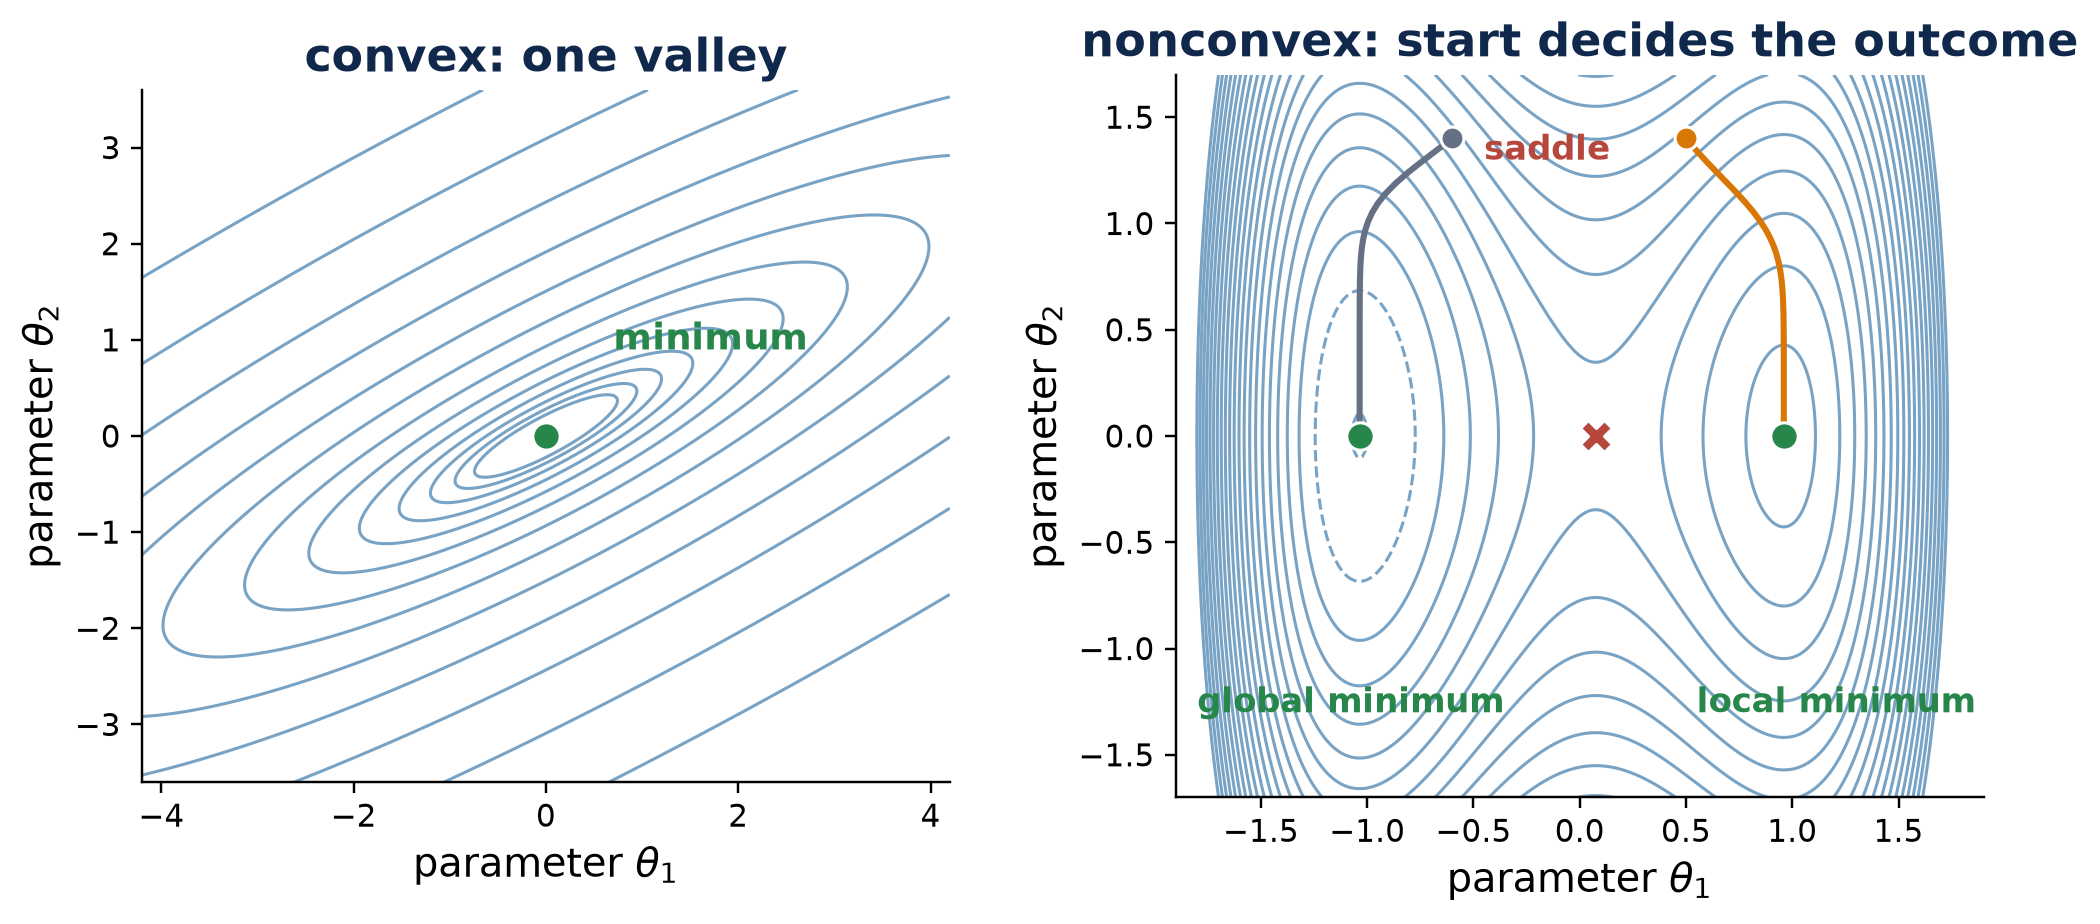
\includegraphics[width=0.98\linewidth,height=0.62\textheight,keepaspectratio]{landscapes.png}
  \begin{itemize}
    \item The contour lines connect parameters with equal loss; the lowest point is the minimum.
    \item Left, \textbf{one valley}: least squares and logistic regression are like this.
    \item Right, \textbf{several valleys} (and a \textbf{saddle}): neural networks are like this.
  \end{itemize}
\end{frame}

\begin{frame}{Minima, Saddles, and What We Can See}
  \begin{center}
  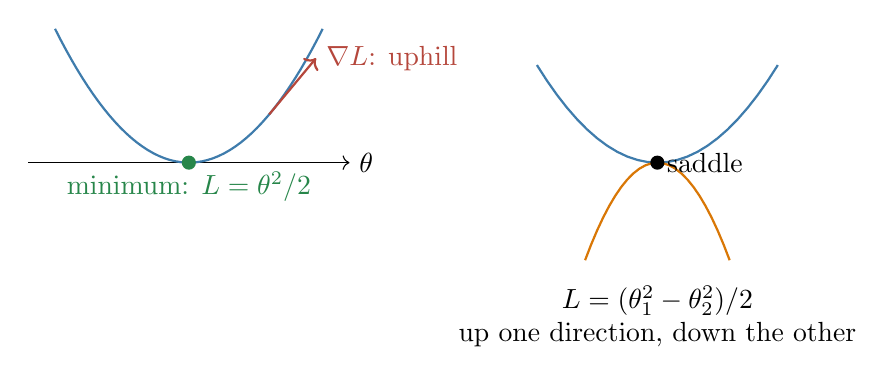
\begin{tikzpicture}[scale=0.85]
    \draw[->] (-2.4,0)--(2.4,0) node[right] {\(\theta\)};
    \draw[courseblue,thick,domain=-2:2,samples=50] plot (\x,{0.5*\x*\x});
    \fill[coursegreen] (0,0) circle (3pt) node[below] {minimum: \(L=\theta^2/2\)};
    \draw[->,coursered,thick] (1.2,0.72)--(1.9,1.56) node[right] {\(\nabla L\): uphill};
    \begin{scope}[xshift=7cm]
      \draw[courseblue,thick,domain=-1.8:1.8] plot (\x,{0.45*\x*\x});
      \draw[courseorange,thick,domain=-1.8:1.8] plot ({0.6*\x},{-0.45*\x*\x});
      \fill (0,0) circle (3pt) node[right] {saddle};
      \node[below,align=center] at (0,-1.7) {\(L=(\theta_1^2-\theta_2^2)/2\)\\up one direction, down the other};
    \end{scope}
  \end{tikzpicture}
  \end{center}
  \[\nabla L=\mathbf0\text{ at both};\qquad H_{ij}=\frac{\partial^2L}{\partial\theta_i\partial\theta_j}.\]
  Positive Hessian eigenvalues give a bowl; mixed signs give a saddle. The Hessian measures how the gradient changes.
\end{frame}

% ------------------------------------------------------------ 2. Gradient descent
\section{Gradient descent}
\sectiondivider{2. Gradient Descent: Walk Downhill}

\begin{frame}{The Gradient Points Uphill}
  \begin{columns}[T]
    \begin{column}{0.5\textwidth}
      The \textbf{gradient} $\nabla L(\boldsymbol\theta)$ lists how fast the loss grows when each
      parameter grows.
      \begin{itemize}
        \item It points in the direction of steepest \emph{increase}.
        \item Its length is the steepness.
        \item So $-\nabla L$ points steepest \emph{downhill}.
      \end{itemize}
    \end{column}
    \begin{column}{0.5\textwidth}
      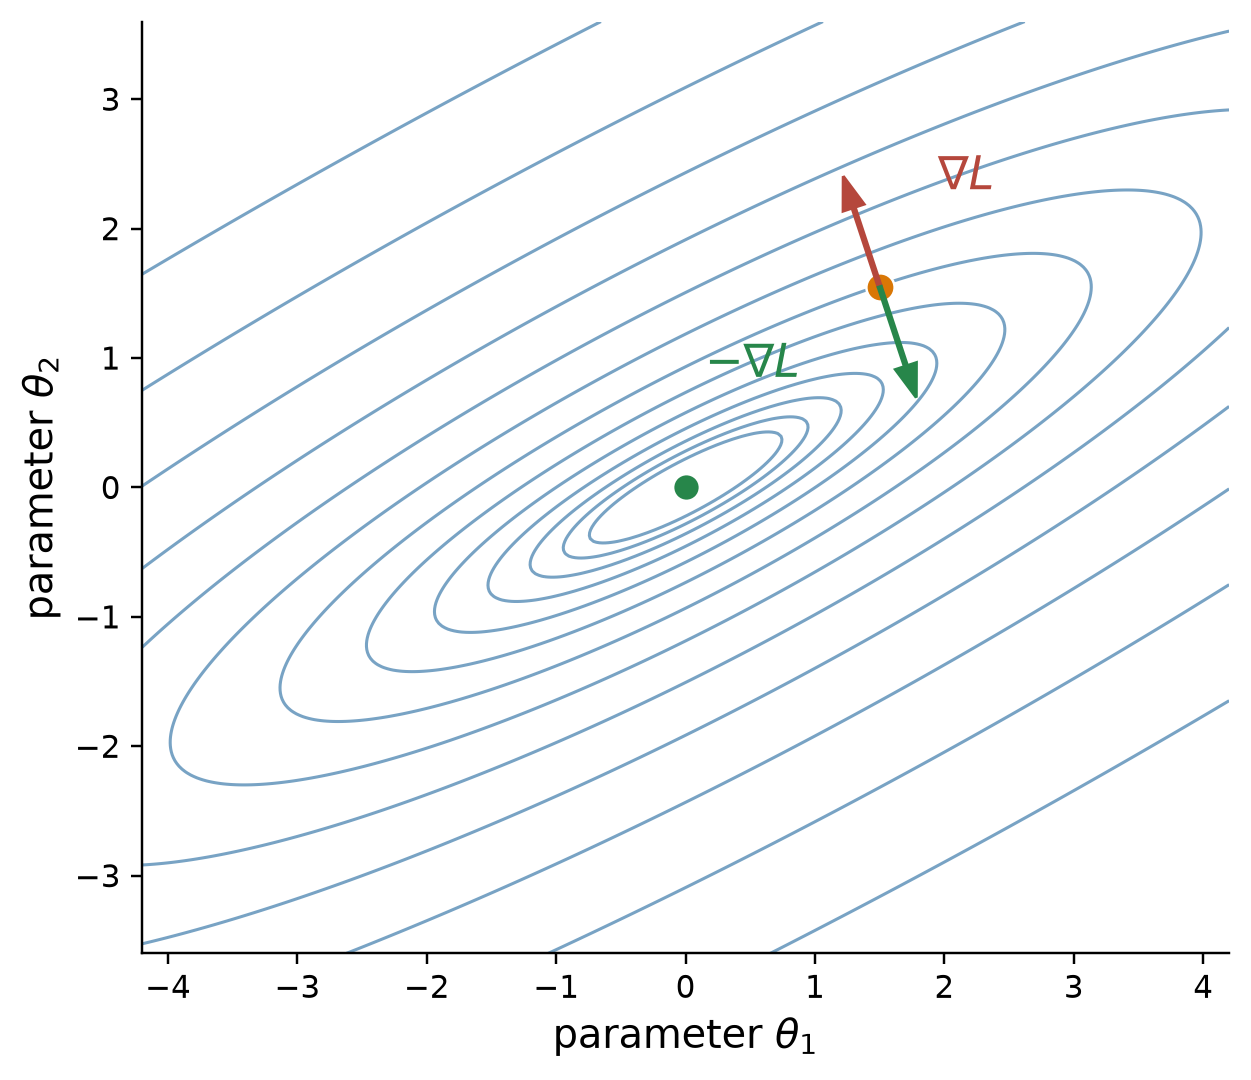
\includegraphics[width=\linewidth,height=0.62\textheight,keepaspectratio]{objective-geometry.png}
    \end{column}
  \end{columns}
  \takeaway{So: to lower the loss, take a step against the gradient.}
\end{frame}

\begin{frame}{The Gradient Descent Update}
  \[
    \boxed{\boldsymbol\theta^{(t+1)}=\boldsymbol\theta^{(t)}-\eta\,\nabla L\bigl(\boldsymbol\theta^{(t)}\bigr)}
  \]
  \begin{itemize}
    \item $\boldsymbol\theta^{(t)}$: the parameters after $t$ updates.
    \item $\eta>0$: the \textbf{learning rate}, how far we step.
    \item Repeat until the loss stops decreasing.
  \end{itemize}
\end{frame}

\begin{frame}{A Worked Example with One Parameter}
  \(L(\theta)=\theta^2\), \(\nabla L=2\theta\); start at \(\theta^{(0)}=3\), \(\eta=0.1\).
  \begin{center}
  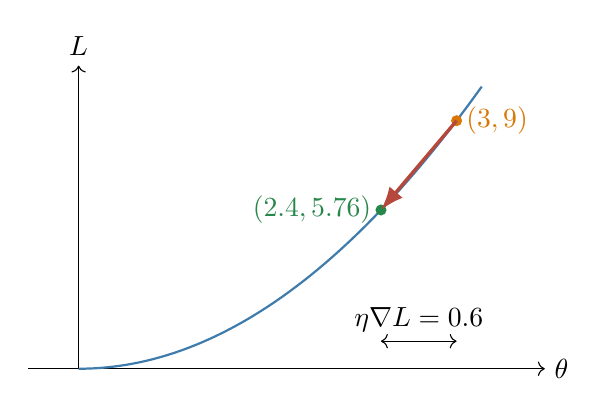
\begin{tikzpicture}[x=1.6cm,y=0.35cm]
    \draw[->] (-0.4,0)--(3.7,0) node[right] {\(\theta\)};
    \draw[->] (0,0)--(0,11) node[above] {\(L\)};
    \draw[courseblue,thick,domain=0:3.2,samples=60] plot (\x,{\x*\x});
    \fill[courseorange] (3,9) circle (2pt) node[right] {\((3,9)\)};
    \fill[coursegreen] (2.4,5.76) circle (2pt) node[left] {\((2.4,5.76)\)};
    \draw[-{Latex},very thick,coursered] (3,9)--(2.4,5.76);
    \draw[<->] (2.4,1)--node[above] {\(\eta\nabla L=0.6\)} (3,1);
  \end{tikzpicture}
  \end{center}
  \[\theta^{(1)}=3-0.1\times6=2.4,\qquad L(2.4)=5.76<9.\]
\end{frame}

\begin{frame}{The Learning Rate Sets the Step Size}
  \centering
  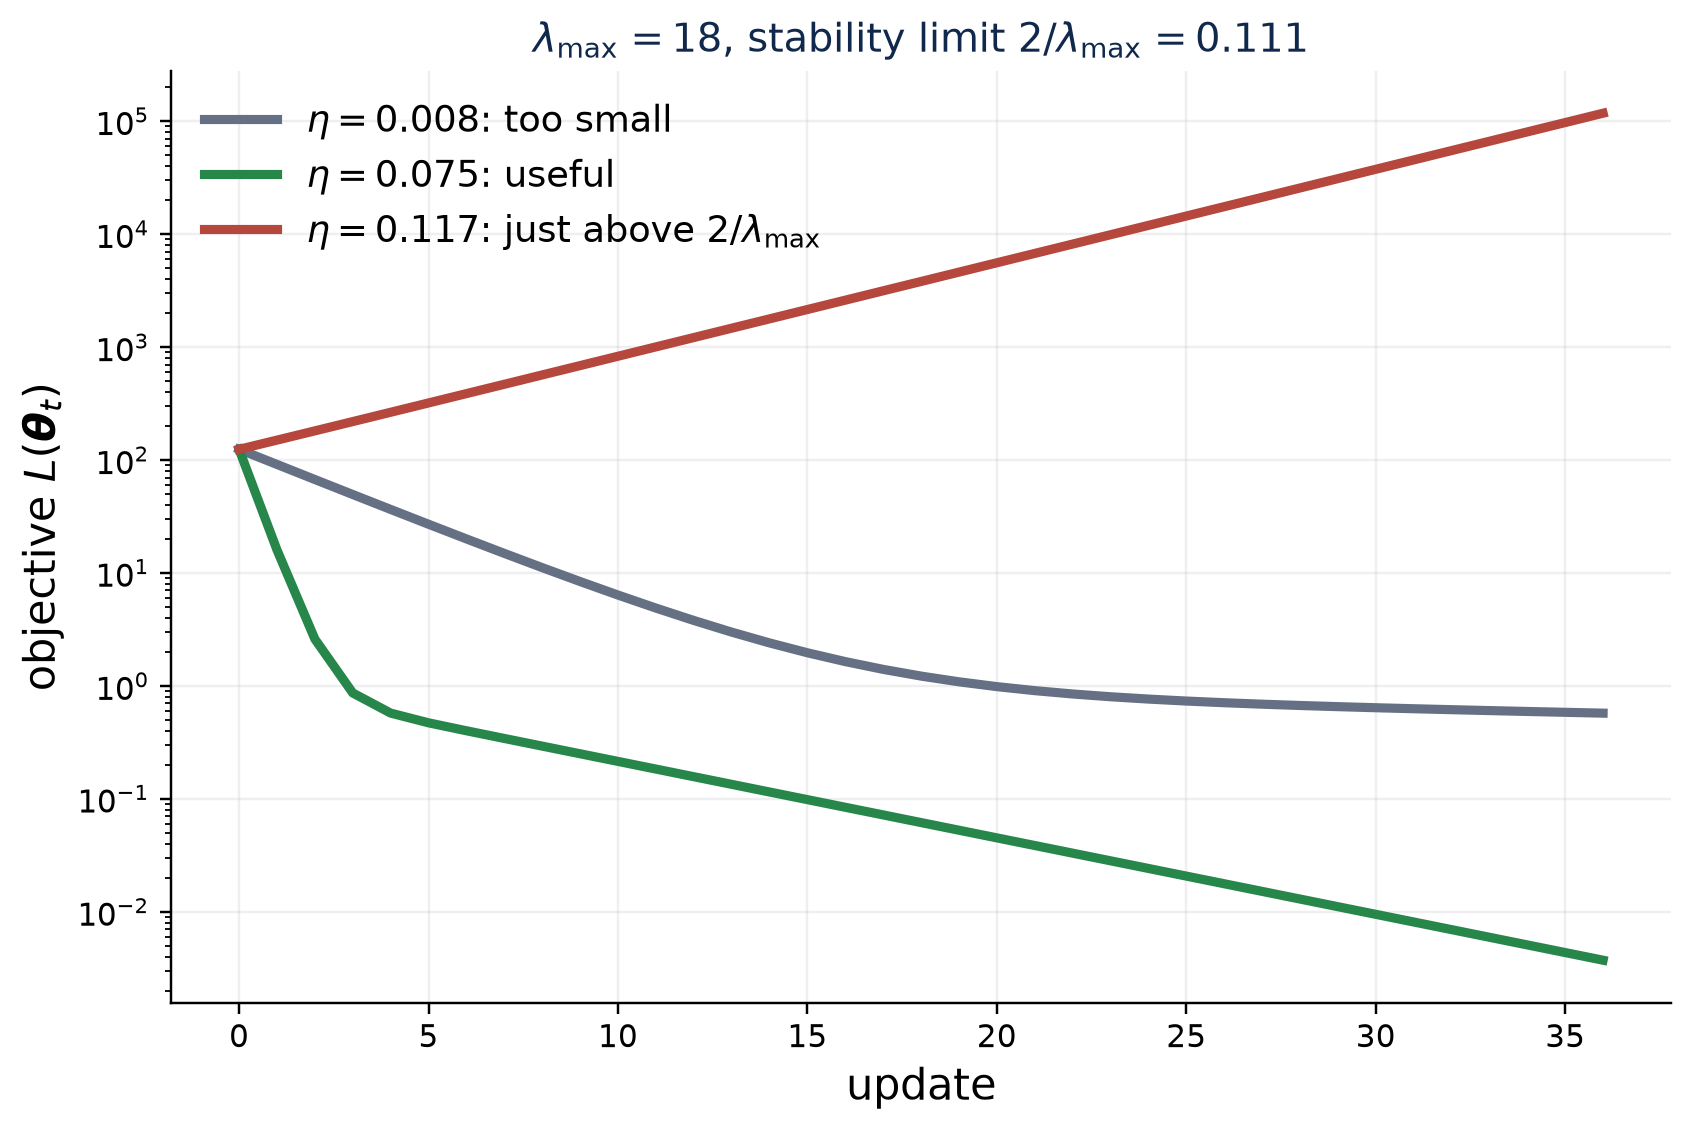
\includegraphics[width=0.7\linewidth,height=0.5\textheight,keepaspectratio]{learning-rates.png}
  \begin{itemize}
    \item Too small: safe but slow. Too large: the steps overshoot and the loss grows.
  \end{itemize}
  \takeaway{So: $\eta$ is the first setting to get right, and the right value depends on the problem.}
\end{frame}

% ------------------------------------------------------------ 3. Curvature
\section{Curvature}
\sectiondivider{3. Curvature: Why One Step Size Does Not Fit All}

\begin{frame}{Slope Is Not Enough: Curvature}
  The slope says which way is down. The \textbf{curvature} says how quickly the slope itself
  changes: a narrow steep bowl has large curvature, a wide flat bowl has small curvature.
  \medskip

  Take $L(\theta)=a\theta^2$, so the update is $\theta\leftarrow(1-2a\eta)\,\theta$. With $\eta=0.3$
  and start $\theta=1$:
  \begin{center}
    \begin{tabular}{lcc}
      \toprule
      & steep bowl, $a=5$ & flat bowl, $a=0.1$ \\
      \midrule
      factor per update $1-2a\eta$ & $-2$ & $0.94$ \\
      $\theta$ after 1, 2, 3 updates & $-2,\ 4,\ -8$ & $0.94,\ 0.88,\ 0.83$ \\
      \bottomrule
    \end{tabular}
  \end{center}
  \takeaway{So: the same $\eta$ explodes on the steep bowl and crawls on the flat one.}
\end{frame}

\begin{frame}{The Hessian Collects the Curvature}
  \[H_{ij}=\frac{\partial^2L}{\partial\theta_i\partial\theta_j},\qquad
    H\mathbf q_j=\lambda_j\mathbf q_j\]
  \[L(\boldsymbol\theta+\boldsymbol\delta)\approx
    L(\boldsymbol\theta)+\nabla L^\top\boldsymbol\delta+	frac12\boldsymbol\delta^\top H\boldsymbol\delta\]
  \begin{itemize}
    \item Eigenvector \(\mathbf q_j\): a curvature direction; \(\lambda_j\): its curvature.
    \item Large positive \(\lambda_j\): steep wall, small stable step.
    \item Small positive \(\lambda_j\): flat floor, slow progress.
    \item Near a nondegenerate minimum, \(H\succ0\) gives a local bowl.
  \end{itemize}
\end{frame}

\begin{frame}{Steep and Flat Together Make a Narrow Valley}
  \small
  \centering
  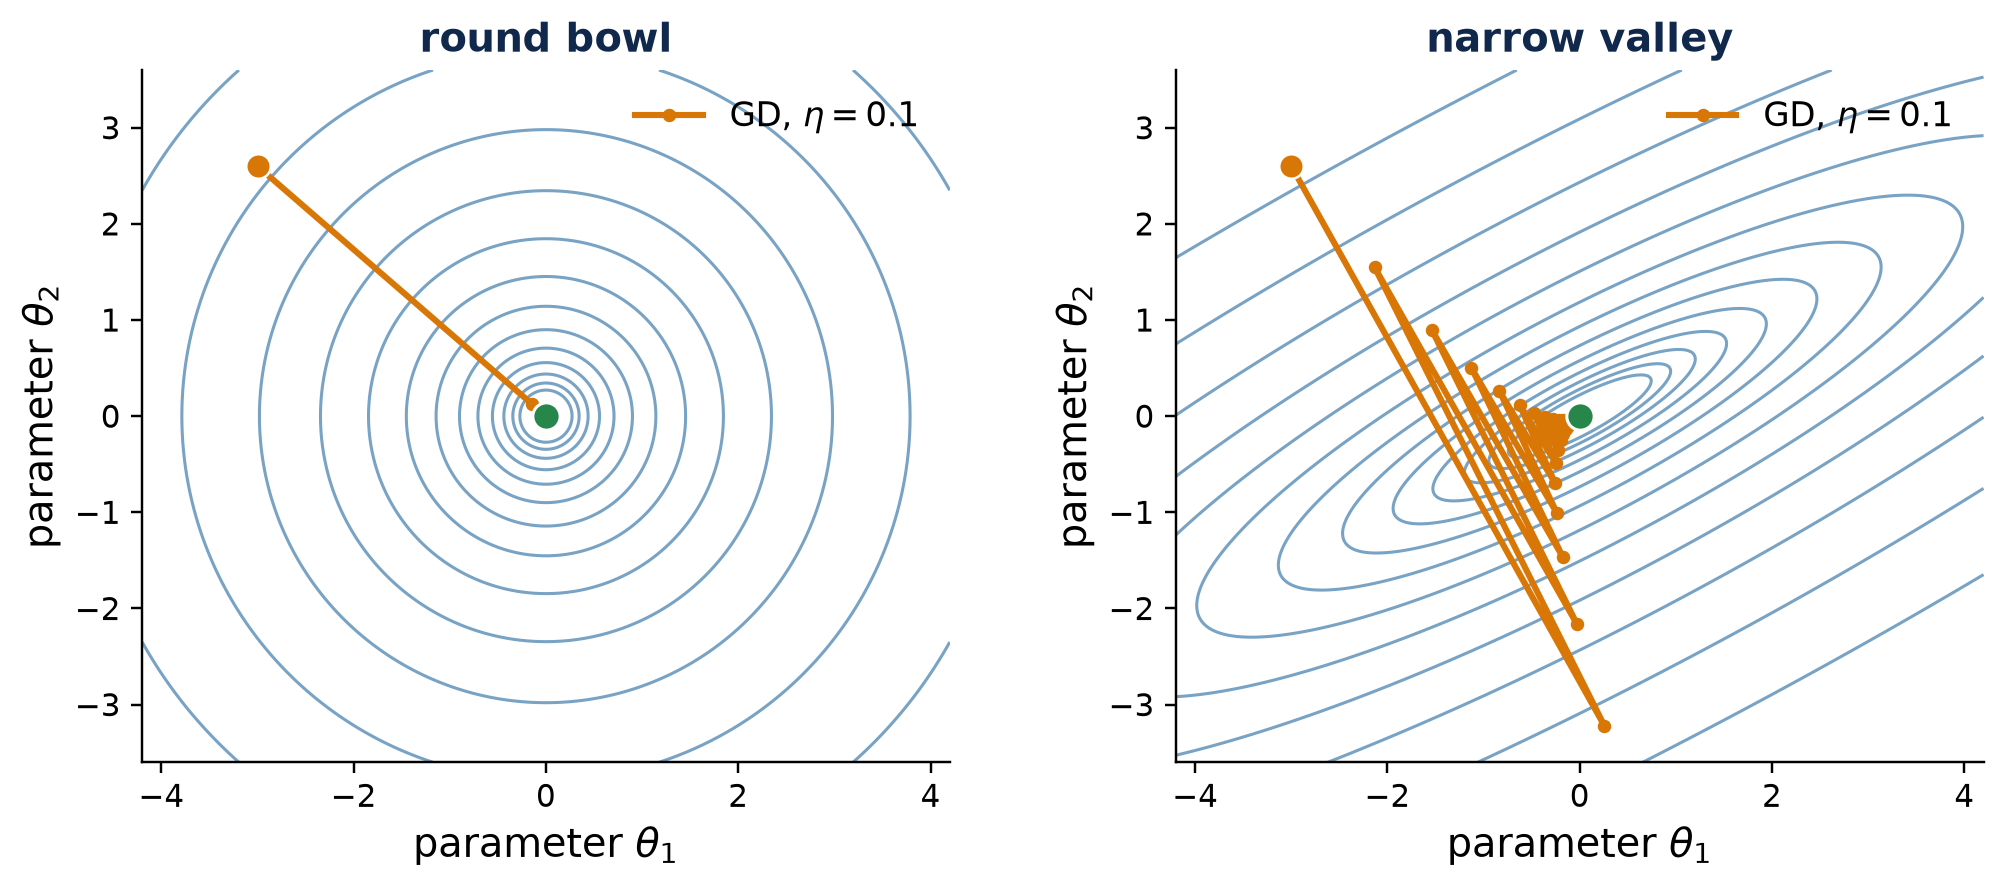
\includegraphics[width=0.90\linewidth,height=0.43\textheight,keepaspectratio]{conditioning.png}
  \[L=\tfrac12\boldsymbol\theta^\top H\boldsymbol\theta,\quad H\succ0,\quad\kappa=\frac{\lambda_{\max}(H)}{\lambda_{\min}(H)}.\]
  \small Round: \(\kappa=1\). Narrow: \(\kappa\gg1\), so steep curvature limits the step.
  \begin{itemize}
    \item In the round bowl one step goes straight to the minimum.
    \item In the narrow valley the steep direction forces a small $\eta$; gradient descent bounces
      across the valley and crawls along it.
  \end{itemize}
\end{frame}

\begin{frame}{Standardizing Inputs Rounds the Valley}
  \[\boxed{x_j^{\mathrm{std}}=\frac{x_j-\mu_j}{s_j}}\qquad(s_j>0)\]
  \begin{itemize}
    \item Fit feature means \(\mu_j\) and standard deviations \(s_j\) on the training set.
    \item Unequal feature units can create unequal curvature; standardization often rounds the valley.
    \item Constant features need separate handling (no division by zero).
    \item Correlations and unequal layer scales can remain; coordinate scaling cannot remove every narrow valley.
  \end{itemize}
  Preprocessing details: supervised-learning lecture.
\end{frame}

% ------------------------------------------------------------ 4. Mini-batches
\section{Mini-batches}
\sectiondivider{4. Mini-Batches: Cheaper, Noisier Gradients}

\begin{frame}{A Mini-Batch Estimates the Gradient}
  \small
  Average the gradient over a random subset $\mathcal B$ of $b$ samples instead:
  \[
    \mathbf g=\frac1b\sum_{i\in\mathcal B}\nabla\ell_i(\boldsymbol\theta)
  \]
  \begin{center}
    \begin{tabular}{lll}
      \toprule
      \textbf{Method} & \textbf{Batch size} $b$ & \textbf{Behavior} \\
      \midrule
      full-batch GD & $n$ & exact gradient, expensive update \\
      SGD (stochastic) & $1$ & very noisy, very cheap update \\
      mini-batch & e.g.\ $32$--$256$ & the usual compromise \\
      \bottomrule
    \end{tabular}
  \end{center}
  An \textbf{update} changes $\boldsymbol\theta$ once. An \textbf{epoch} is one pass over the data:
  with $n=1000$ and $b=50$ it takes $20$ updates.
\end{frame}

\begin{frame}{Noise Buys Speed and Costs Precision}
  \small
  \centering
  \[\underbrace{\nabla L=\frac1n\sum_{i=1}^n\nabla\ell_i}_{\text{full batch: exact}}\qquad\underbrace{\mathbf g=\frac1b\sum_{i\in\mathcal B}\nabla\ell_i}_{\text{mini-batch: cheap, noisy}}\]
  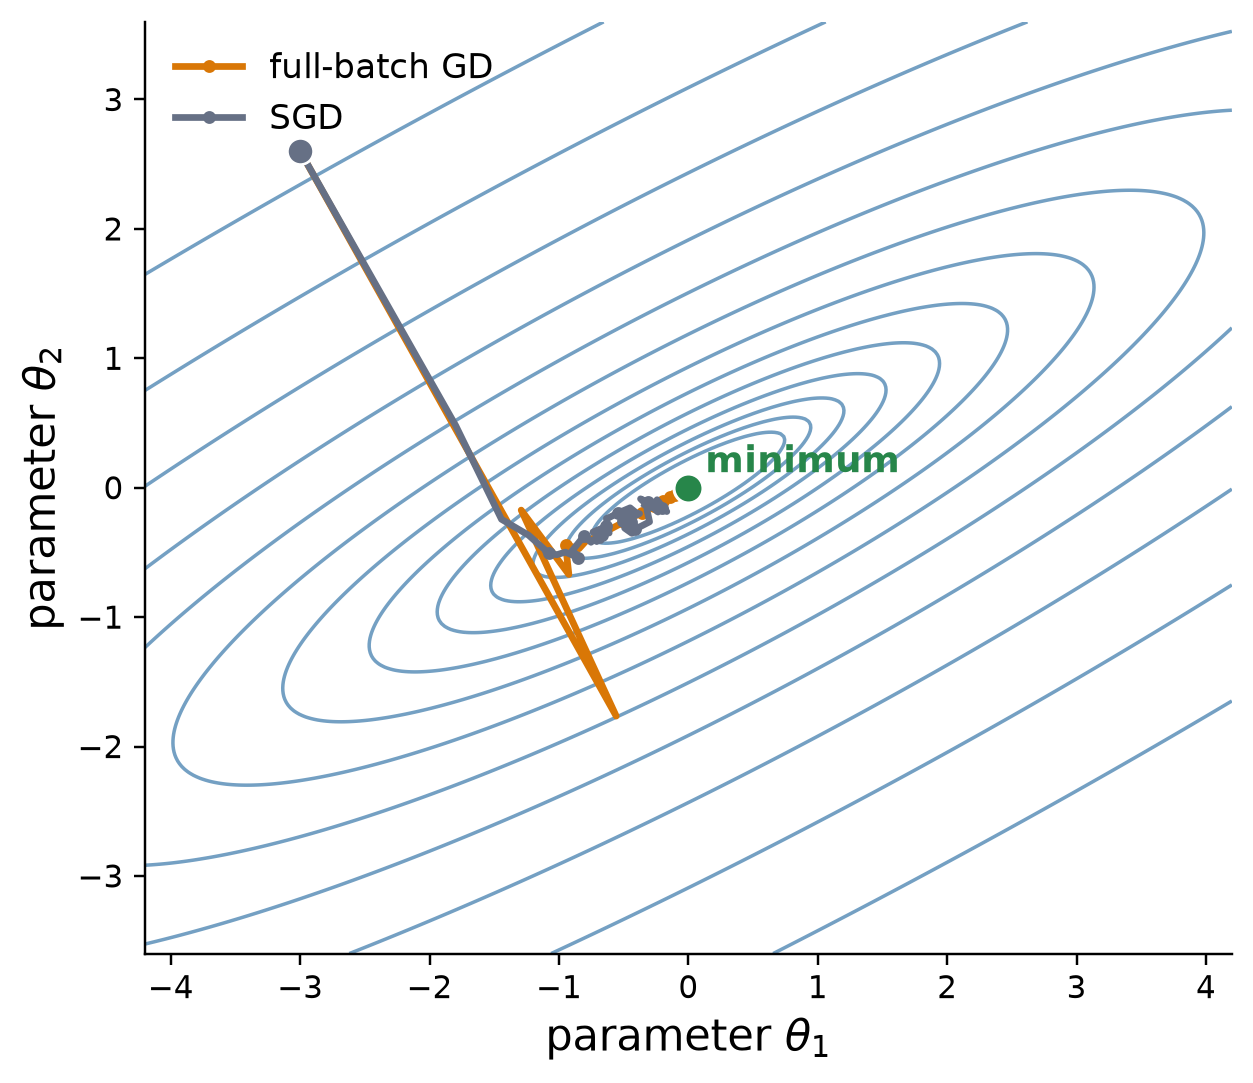
\includegraphics[width=0.86\linewidth,height=0.30\textheight,keepaspectratio]{gd-vs-sgd.png}
  \begin{itemize}
    \item Mini-batch paths wander but head the right way, at a fraction of the cost per update.
    \item With a constant $\eta$ they never settle exactly; a larger batch gives less noise.
  \end{itemize}

\end{frame}

\begin{frame}{Shrink the Learning Rate to Settle Down}
  \centering
  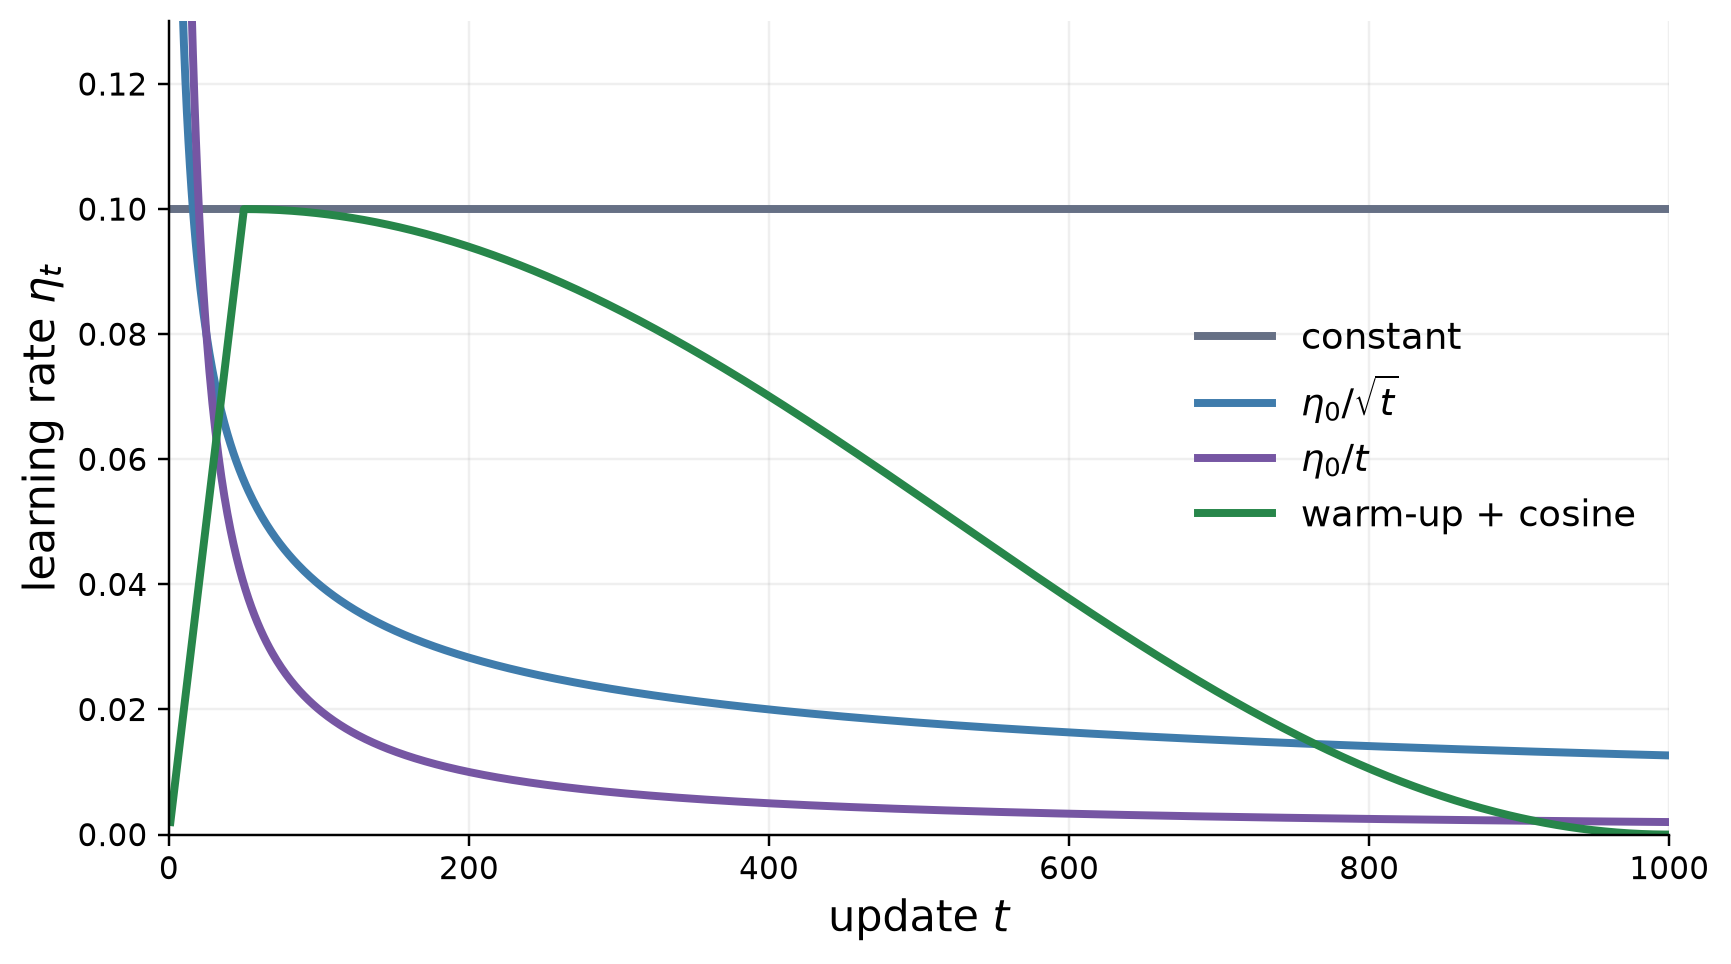
\includegraphics[width=0.7\linewidth,height=0.46\textheight,keepaspectratio]{schedules.png}
  \begin{itemize}
    \item A \textbf{schedule} changes $\eta$ during training: large steps early, small steps late.
    \item \textbf{Warm-up} starts small and grows first, because early gradients can be erratic.
  \end{itemize}
  \takeaway{So: decay $\eta$ over training; the noise floor shrinks with it.}
\end{frame}

% ------------------------------------------------------------ 5. Momentum
\section{Momentum}
\sectiondivider{5. Momentum: Remember the Direction}

\begin{frame}{The Momentum Update}
  \[
    \mathbf v^{(t)}=\beta\,\mathbf v^{(t-1)}+\mathbf g^{(t)},
    \qquad
    \boxed{\boldsymbol\theta^{(t+1)}=\boldsymbol\theta^{(t)}-\eta\,\mathbf v^{(t)}}
  \]
  \begin{itemize}
    \item $\mathbf v$ is the velocity: a running sum of past gradients.
    \item $\beta\in[0,1)$ is how much is remembered; $\beta=0$ gives plain gradient descent.
  \end{itemize}
  If the gradient stays at $1$ and $\beta=0.9$, then $\mathbf v=1,\ 1.9,\ 2.71,\ \dots\to10$:
  steady directions end up with steps $1/(1-\beta)=10$ times larger.
  \takeaway{So: momentum speeds up exactly the directions where the gradient is consistent.}
\end{frame}

\begin{frame}{Momentum in the Valley}
  \small
  \centering
  \[\mathbf v^{(t)}=\beta\mathbf v^{(t-1)}+\mathbf g^{(t)},\qquad\boldsymbol\theta^{(t+1)}=\boldsymbol\theta^{(t)}-\eta\mathbf v^{(t)}\]
  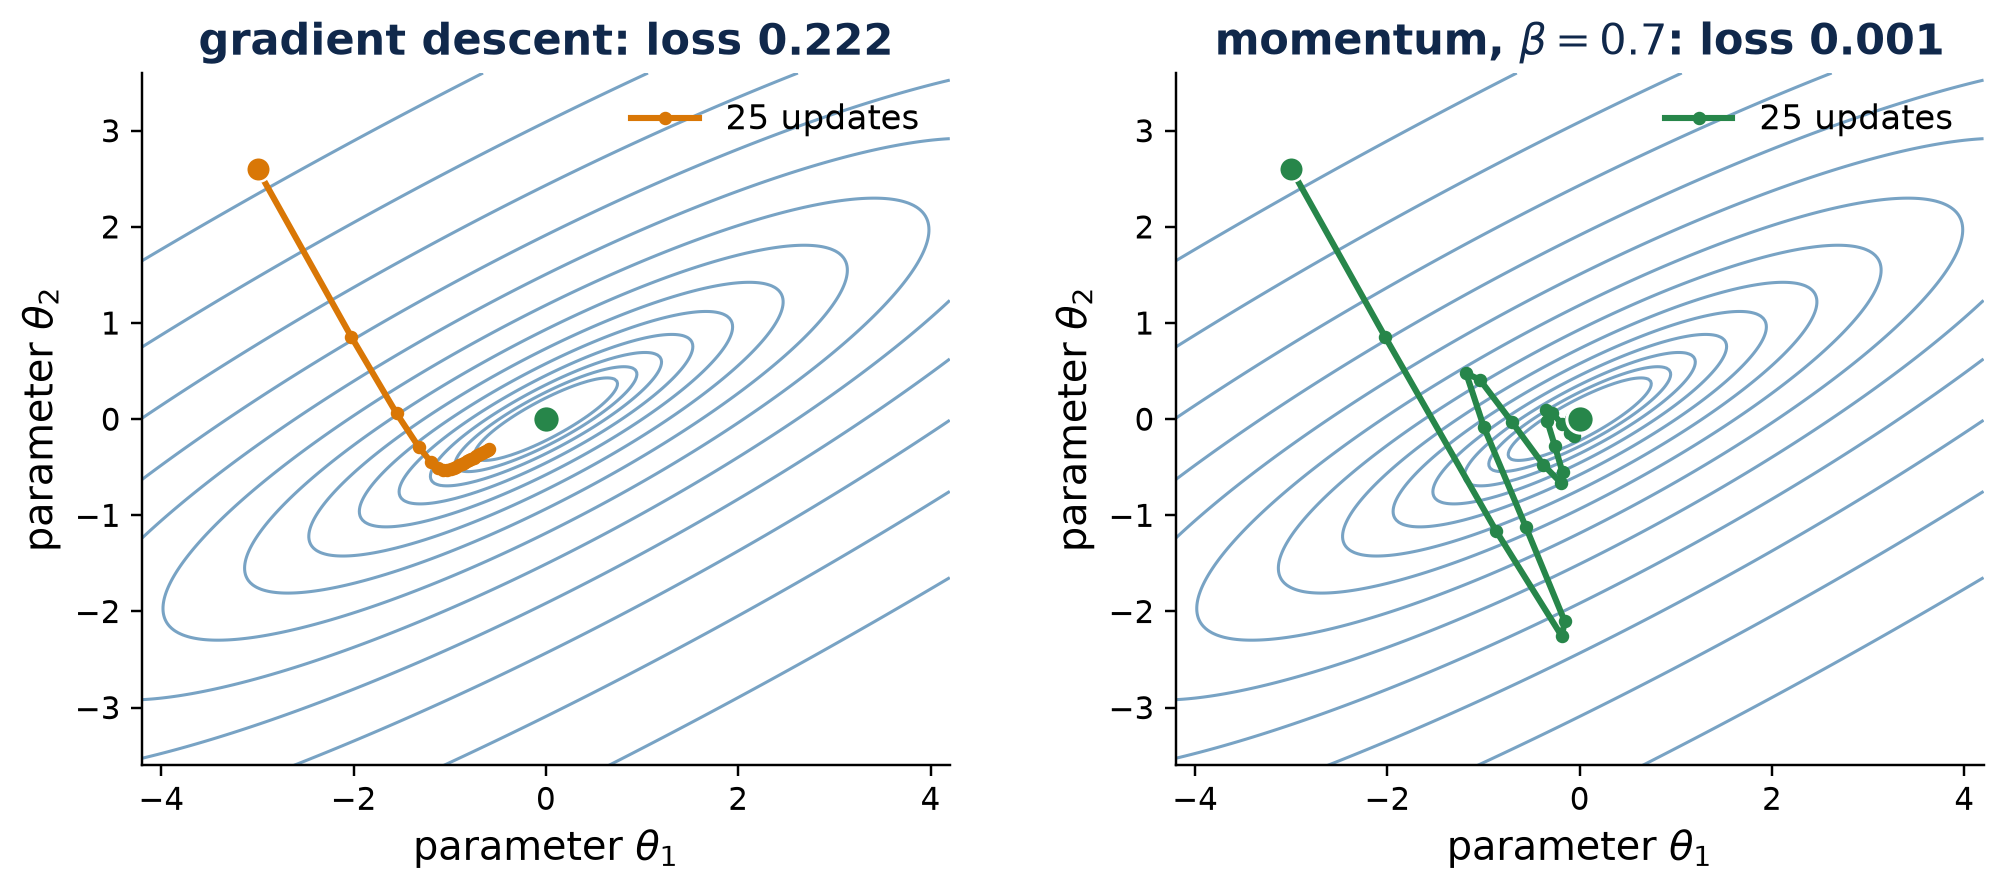
\includegraphics[width=0.90\linewidth,height=0.43\textheight,keepaspectratio]{momentum-paths.png}
  \begin{itemize}
    \item Same valley, same $\eta$, same 25 updates: gradient descent is still crawling,
      momentum has arrived (and overshoots a little on the way).
  \end{itemize}
  \takeaway{So: momentum helps in narrow valleys; $\eta$ and $\beta$ must be tuned together.}
\end{frame}

% ------------------------------------------------------------ 6. Per-parameter
\section{Per-parameter step sizes}
\sectiondivider{6. Per-Parameter Step Sizes: AdaGrad and RMSProp}

\begin{frame}{A New Problem: Parameters on Different Scales}
  Parameter A has gradients of size about $10$; parameter B about $0.1$. With one $\eta$:
  \begin{center}
    \begin{tabular}{lccc}
      \toprule
      & gradient & step with $\eta=0.01$ \\
      \midrule
      A & $10$ & $0.1$ (big) \\
      B & $0.1$ & $0.001$ (negligible) \\
      \bottomrule
    \end{tabular}
  \end{center}
  Choose $\eta$ for A and B barely moves; choose it for B and A overshoots.
  \takeaway{So: we want each parameter to take steps of a sensible size on its own scale.}
\end{frame}

\begin{frame}{AdaGrad: Divide by the History of Gradient Size}
  \small
  \[
    \mathbf s^{(t)}=\mathbf s^{(t-1)}+\mathbf g^{(t)}\odot\mathbf g^{(t)}
  \]
  \[
    \boldsymbol\theta^{(t+1)}=\boldsymbol\theta^{(t)}-\eta\,\frac{\mathbf g^{(t)}}{\sqrt{\mathbf s^{(t)}}+\varepsilon}
  \]
  $\mathbf s$ adds up the squared gradient of each parameter ($\odot$ is element-wise product),
  so $\sqrt{\mathbf s}$ is the accumulated gradient magnitude of that parameter. Example, gradients
  $10,8,9$ for A and $0.1,0.08,0.09$ for B:
  \begin{center}
    \begin{tabular}{lccc}
      \toprule
      update & 1 & 2 & 3 \\
      \midrule
      A: $g/\sqrt s$ & $1.00$ & $0.62$ & $0.58$ \\
      B: $g/\sqrt s$ & $1.00$ & $0.62$ & $0.58$ \\
      \bottomrule
    \end{tabular}
  \end{center}
  Both parameters now take steps of the same size. $\varepsilon$ ($10^{-8}$) only avoids dividing by zero.
  \takeaway{So: dividing by the gradient's own scale removes the scale difference.}
\end{frame}

\begin{frame}{AdaGrad Slows Down Forever}
  $\mathbf s$ only ever grows, so $\sqrt{\mathbf s}$ only grows and the steps only shrink.
  \begin{itemize}
    \item Early on this is helpful; late in training it can stall before the minimum is reached.
    \item Fix: forget old gradients, so $\mathbf s$ tracks only the recent size.
  \end{itemize}
  \textbf{RMSProp} replaces the sum by a moving average:
  \[
    \mathbf s^{(t)}=\rho\,\mathbf s^{(t-1)}+(1-\rho)\,\mathbf g^{(t)}\odot\mathbf g^{(t)}
  \]
  \[\boldsymbol\theta^{(t+1)}=\boldsymbol\theta^{(t)}-\eta\,\frac{\mathbf g^{(t)}}{\sqrt{\mathbf s^{(t)}}+\varepsilon}.\]
  $\rho$ (typically $0.9$) sets the memory; old large gradients fade rather than shrinking all later steps.
  \takeaway{So: RMSProp keeps AdaGrad's per-parameter scaling without the permanent slowdown.}
\end{frame}

% ------------------------------------------------------------ 7. Adam
\section{Adam}
\sectiondivider{7. Adam: Momentum and Per-Parameter Step Sizes Together}

\begin{frame}{Adam Combines Both Ideas}
  \centering
  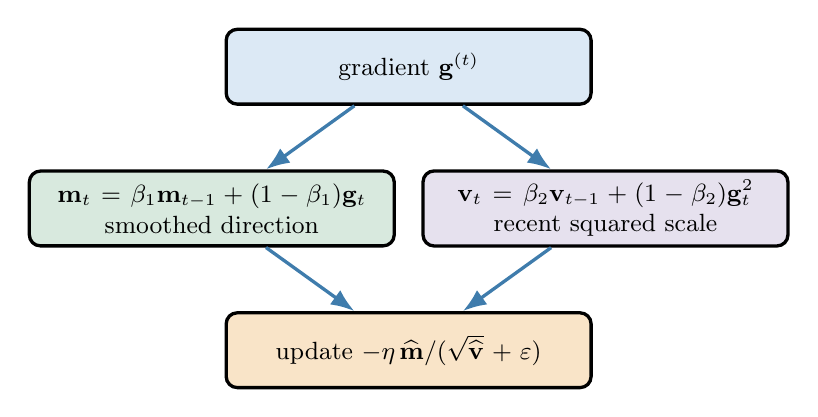
\begin{tikzpicture}[
    box/.style={draw,rounded corners,text width=4.4cm,minimum height=0.95cm,align=center,very thick,font=\small},
    flow/.style={-{Latex[length=3mm]},very thick,courseblue}
  ]
    \node[box,fill=courselightblue] (gradient) at (0,0) {gradient $\mathbf g^{(t)}$};
    \node[box,fill=coursegreen!18] (first) at (-2.5,-1.8) {$\mathbf m_t=\beta_1\mathbf m_{t-1}+(1-\beta_1)\mathbf g_t$\\smoothed direction};
    \node[box,fill=coursepurple!18] (second) at (2.5,-1.8) {$\mathbf v_t=\beta_2\mathbf v_{t-1}+(1-\beta_2)\mathbf g_t^2$\\recent squared scale};
    \node[box,fill=courselightorange] (update) at (0,-3.6) {update $-\eta\,\widehat{\mathbf m}/(\sqrt{\widehat{\mathbf v}}+\varepsilon)$};
    \draw[flow] (gradient) -- (first);
    \draw[flow] (gradient) -- (second);
    \draw[flow] (first) -- (update);
    \draw[flow] (second) -- (update);
  \end{tikzpicture}
  \takeaway{So: Adam steps in the smoothed direction, measured in each parameter's own units.}
\end{frame}

\begin{frame}{The Adam Update}
  \[
    \mathbf m^{(t)}=\beta_1\mathbf m^{(t-1)}+(1-\beta_1)\,\mathbf g^{(t)}
    \qquad\text{(direction: momentum)}
  \]
  \[
    \mathbf v^{(t)}=\beta_2\mathbf v^{(t-1)}+(1-\beta_2)\,\mathbf g^{(t)}\odot\mathbf g^{(t)}
    \qquad\text{(scale: RMSProp)}
  \]
  \[
    \widehat{\mathbf m}^{(t)}=\frac{\mathbf m^{(t)}}{1-\beta_1^{\,t}},\qquad
    \widehat{\mathbf v}^{(t)}=\frac{\mathbf v^{(t)}}{1-\beta_2^{\,t}}
  \]
  \[
    \boxed{\boldsymbol\theta^{(t+1)}=\boldsymbol\theta^{(t)}-\eta\,
      \frac{\widehat{\mathbf m}^{(t)}}{\sqrt{\widehat{\mathbf v}^{(t)}}+\varepsilon}}
  \]
  Common defaults: $\beta_1=0.9$, $\beta_2=0.999$, $\varepsilon=10^{-8}$.
  \takeaway{So: $\mathbf m$ is momentum, $\mathbf v$ is RMSProp, and the hats are a start-up correction (next frame).}
\end{frame}

\begin{frame}{Bias Correction Fixes the Cold Start}
  $\mathbf m$ and $\mathbf v$ start at $0$, so the first averages are too small. Example: the gradient
  is always $2$.
  \begin{center}
    \begin{tabular}{lcc}
      \toprule
      after update 1 & $\mathbf m$ & $\mathbf v$ \\
      \midrule
      raw average & $0.1\cdot2=0.2$ & $0.001\cdot4=0.004$ \\
      divided by $1-\beta^{\,1}$ & $0.2/0.1=2$ & $0.004/0.001=4$ \\
      \bottomrule
    \end{tabular}
  \end{center}
  The corrected values are the true ones ($2$ and $2^2$), so the first step is
  $\eta\cdot2/\sqrt4=\eta$ instead of the uncorrected step of approximately $3.16\eta$. The correction fades as $t$ grows.
  \takeaway{So: the hats make Adam's very first steps correctly normalized despite zero-initialized moment estimates.}
\end{frame}

% ------------------------------------------------------------ 8. Why Adam
\section{Why Adam}
\sectiondivider{8. Why Adam: A Fair Experiment}

\begin{frame}{The Test: Same Budget, Each Method Tuned}
  \small
  \begin{center}
  \begin{tabular}{@{}lp{8.0cm}@{}}
    \toprule
    Task & Two-input smooth-curve regression; noisy samples; two hidden layers, 24 tanh units each.\\
    Data & 256 training and 512 test samples.\\
    Budget & 40 epochs, batch size 32; average over 5 starts.\\
    Controls & Same data, initialization and batch order for all methods.\\
    Methods & GD; momentum (\(\beta=0.9\)); RMSProp (\(\rho=0.9\)); Adam (defaults).\\
    Tuning & Each method searches learning rates \(10^{-4}\) to \(1\) on a log grid.\\
    Scale test & Second input: same scale, or \(50\) times smaller.\\
    \bottomrule
  \end{tabular}
  \end{center}
  Test loss selects the rate: this is an illustrative comparison, not an unbiased final evaluation.
\end{frame}

\begin{frame}{Result: Test Loss against Learning Rate}
  \centering
  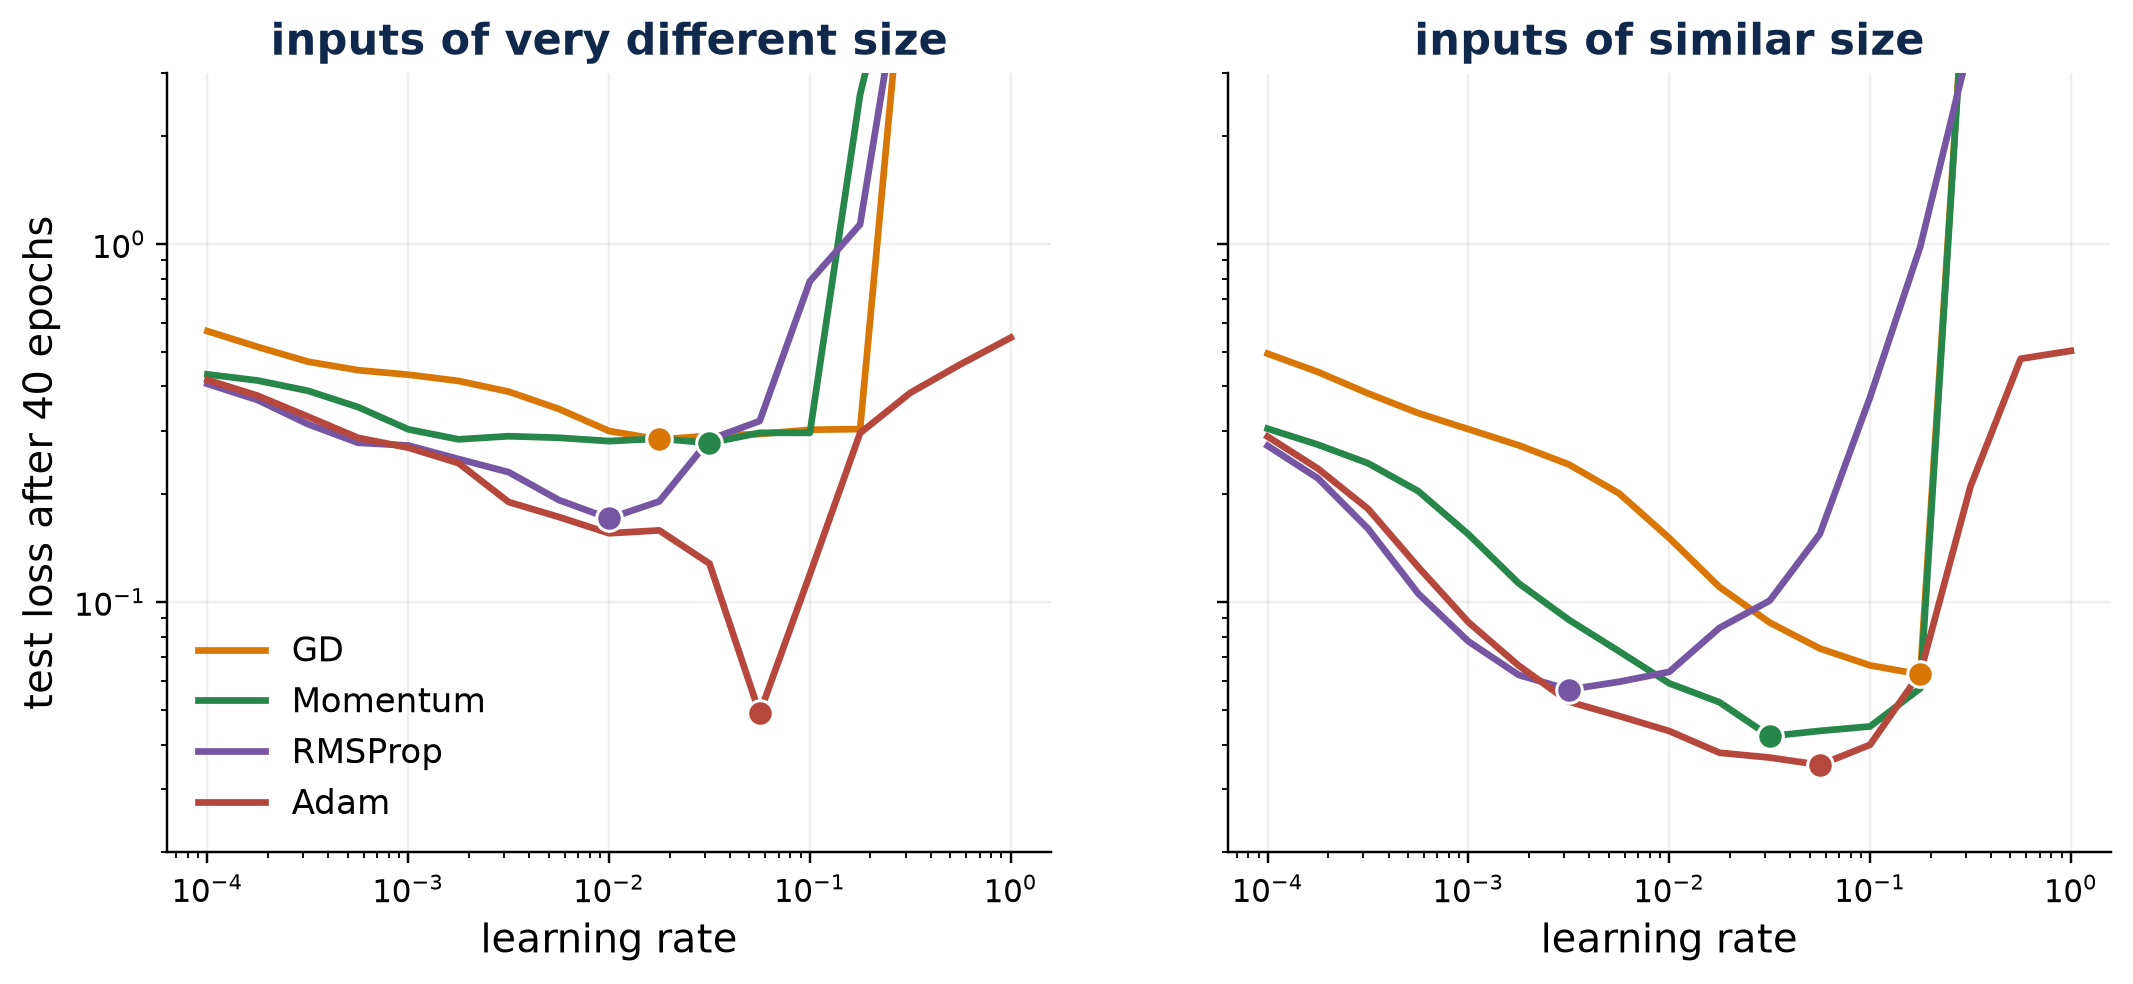
\includegraphics[width=0.98\linewidth,height=0.56\textheight,keepaspectratio]{adam-tuning.png}
  \begin{itemize}
    \item Each curve is one method; its lowest point (the dot) is that method tuned.
    \item Adam's dot is lowest in both versions, by a wide margin when input sizes differ.
  \end{itemize}
\end{frame}

\begin{frame}{Training Curves at Each Method's Best Rate}
  \small
  \centering
  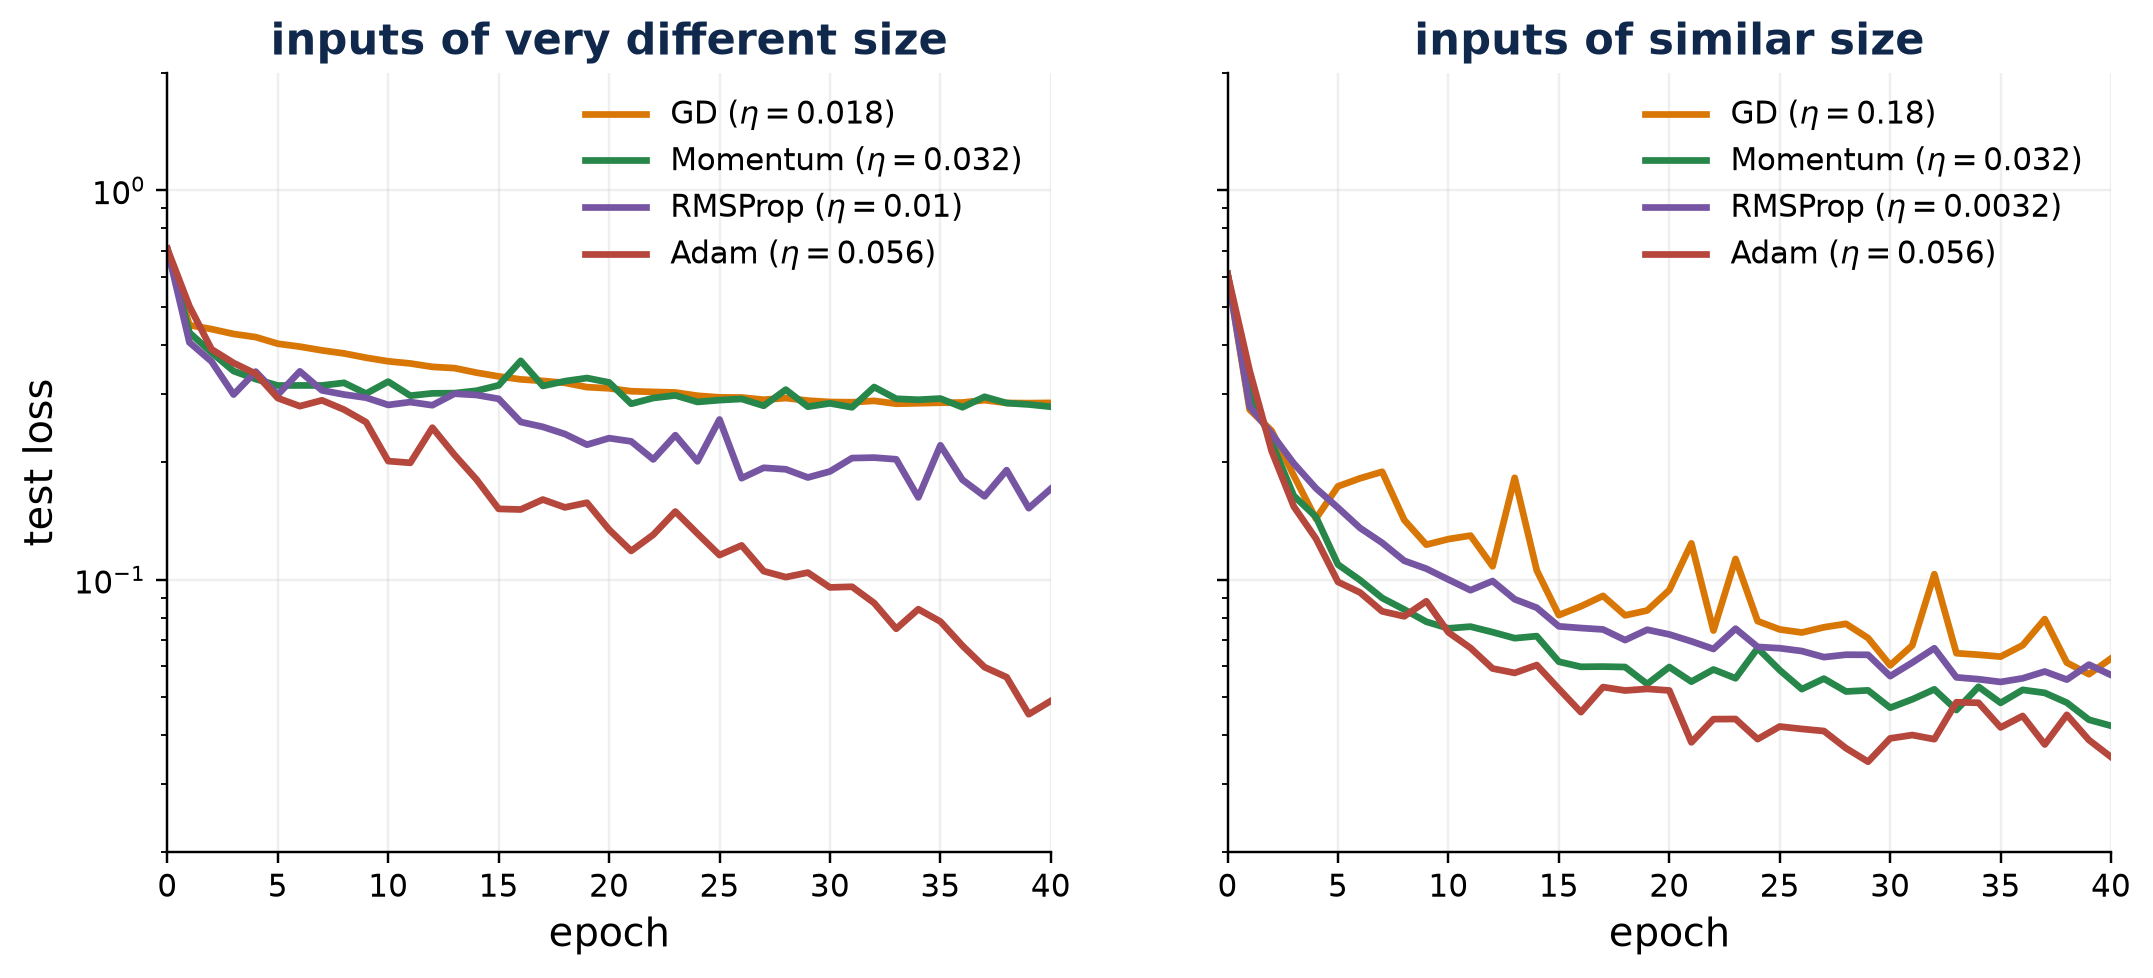
\includegraphics[width=0.98\linewidth,height=0.56\textheight,keepaspectratio]{adam-curves.png}
  \begin{itemize}
    \item Unequal scales (left): Adam keeps improving while GD and momentum stall. Its final test loss is about $6$ times smaller than theirs and $3.5$ times smaller than RMSProp's.
  \end{itemize}
  \takeaway{So: the advantage is not only at the end; Adam gets there faster.}
\end{frame}

\begin{frame}{Why Adam Wins Here, and What This Does Not Show}
  \[\text{tiny input}\ \longrightarrow\ \text{small gradients}
    \ \longrightarrow\ \text{slow unscaled updates}\]
  \begin{itemize}
    \item \textbf{Mechanism:} RMSProp rescales coordinates; Adam also smooths directions.
    \item \textbf{Alternative:} standardize inputs; internal scale differences can remain.
    \item \textbf{Limit:} per-coordinate scaling cannot fully correct rotated valleys.
    \item \textbf{Evidence:} one small task; similar scales give a smaller gap and competitive tuned momentum.
    \item \textbf{Caveat:} rates were selected using test loss; a separate held-out evaluation is needed for an unbiased estimate.
  \end{itemize}
\end{frame}

% ------------------------------------------------------------ 9. Practice
\section{In practice}
\sectiondivider{9. What to Use in Practice}

\begin{frame}{A Practical Recipe}
  \centering
  \small
  \renewcommand{\arraystretch}{1.2}
  \begin{tabular}{@{}>{\raggedright\arraybackslash}p{2.4cm}>{\raggedright\arraybackslash}p{3.8cm}>{\raggedright\arraybackslash}p{4.3cm}@{}}
    \toprule
    \textbf{Method} & \textbf{Good for} & \textbf{Watch for} \\
    \midrule
    GD / SGD & simple baseline, well-scaled problems & slow in narrow valleys; noise floor \\
    SGD + momentum & well-scaled problems, careful tuning & tune $\eta$ and $\beta$ together \\
    Adam & default for neural networks; uneven scales & still needs a good $\eta$; decay it late in training \\
    \bottomrule
  \end{tabular}

  \normalsize
  \medskip
  \begin{itemize}
    \item Start with Adam and a learning rate near $10^{-3}$; search $\eta$ on a log grid.
    \item Standardize the inputs; decay the learning rate; watch the loss for spikes.
  \end{itemize}
\end{frame}

\begin{frame}{What Optimization Does Not Do}
  \begin{itemize}
    \item Gradients of a network's loss come from backpropagation (neural-networks lecture).
    \item Where training ends depends on the start, the step rule, and the schedule.
    \item A small training loss does not guarantee a small error on new data: that is the
      subject of the generalization lecture.
  \end{itemize}
  \takeaway{So: optimization finds low-loss parameters; whether they generalize is a separate question.}
\end{frame}

% ------------------------------------------------------------ Appendix
\appendix
\sectiondivider{Appendix: Optional Depth}

\begin{frame}{Convex Losses Have One Minimum}
  $L$ is \textbf{convex} if the line between any two points of its graph lies above the graph:
  \[
    L(\lambda\mathbf a+(1-\lambda)\mathbf b)\le\lambda L(\mathbf a)+(1-\lambda)L(\mathbf b),\qquad\lambda\in[0,1].
  \]
  \begin{itemize}
    \item For a convex $L$, any point with $\nabla L=\mathbf 0$ is a global minimum.
    \item Least squares and the cross-entropy of logistic regression are convex.
    \item A twice-differentiable $L$ is convex exactly when its Hessian is positive semidefinite everywhere.
    \item Neural-network losses are not convex.
  \end{itemize}
\end{frame}

\begin{frame}{Step-Size Limit on a Quadratic Bowl (Special Case)}
  \textbf{Exact scope:} \(L=\tfrac12\boldsymbol\theta^\top H\boldsymbol\theta\), \(H\succ0\).
  \[e_{j,t+1}=(1-\eta\lambda_j)e_{j,t},\qquad
    \text{convergence}\iff0<\eta<\frac{2}{\lambda_{\max}}\]
  \[\eta_\star=\frac{2}{\lambda_{\min}+\lambda_{\max}},\qquad
    \frac{\|\mathbf e_{t+1}\|_2}{\|\mathbf e_t\|_2}\le\frac{\kappa-1}{\kappa+1},\quad
    \kappa=\frac{\lambda_{\max}}{\lambda_{\min}}\]
  \begin{itemize}
    \item General smooth loss: quadratic behavior is a \textbf{local approximation} near a nondegenerate minimum.
    \item Global sufficient descent bound: \(0<\eta<2/M\) when \(\nabla L\) is \(M\)-Lipschitz; this alone does not imply convergence to a global minimum.
  \end{itemize}
\end{frame}

\begin{frame}{Conditioning Sets the Iteration Count (Quadratic Case)}
  \centering
  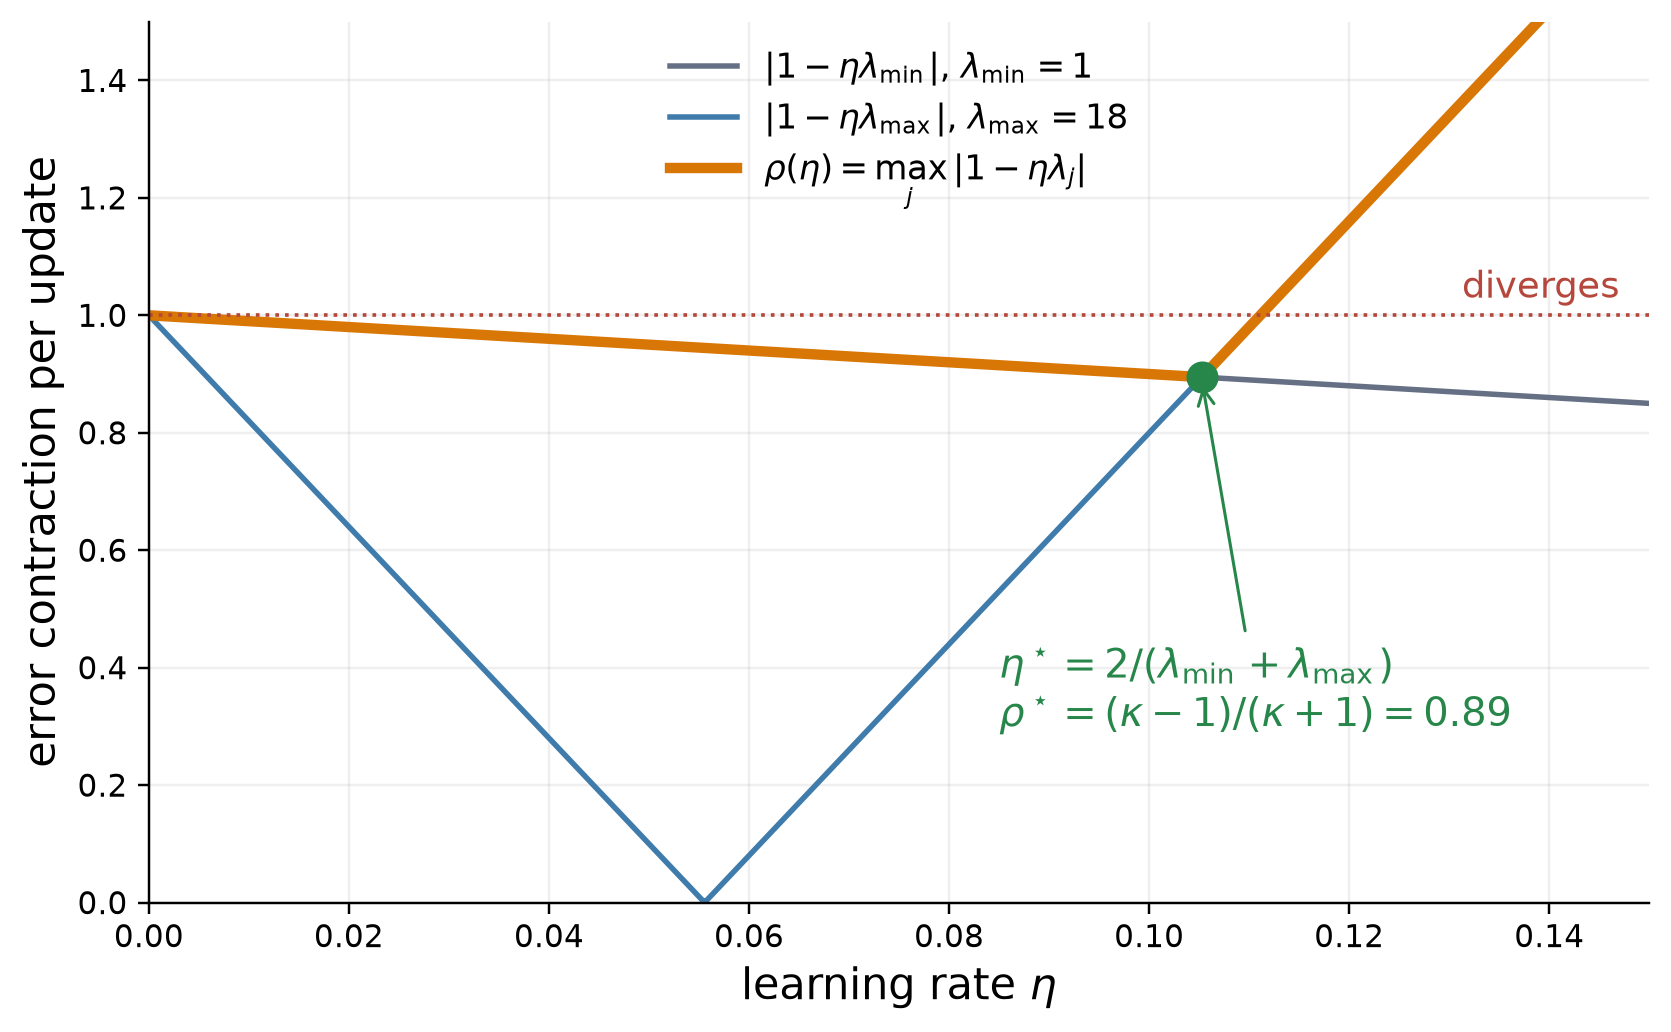
\includegraphics[width=0.78\linewidth,height=0.6\textheight,keepaspectratio]{contraction.png}

  \small
  Contraction per update is $\max_j|1-\eta\lambda_j|$, smallest when the two extreme
  directions contract equally. Reducing the error by a factor $\varepsilon$ takes about
  $\tfrac{\kappa}{2}\ln\tfrac1\varepsilon$ updates for gradient descent.
\end{frame}

\begin{frame}{Mini-Batch Gradients: Unbiased, with Variance $1/b$}
  For a batch of size $b$ drawn uniformly and independently from the $n$ samples,
  \[
    \mathbb E[\mathbf g]=\nabla L(\boldsymbol\theta),\qquad
    \operatorname{Var}(\mathbf g)=\frac1b\operatorname{Var}\bigl(\nabla\ell_i\bigr).
  \]
  \begin{itemize}
    \item \emph{Unbiased}: on average the estimate equals the exact gradient.
    \item Doubling the batch halves the variance but doubles the cost per update.
    \item Per-sample gradients do not vanish at the minimum, so a constant $\eta$ leaves a noise floor.
  \end{itemize}
\end{frame}

\begin{frame}{Learning-Rate Schedule Formulas}
  \begin{align*}
    \text{decay: }&\eta_t=\frac{\eta_0}{t^{\alpha}}\\
    \text{warm-up: }&\eta_t=\eta_{\max}\frac{t}{t_w}\quad(t\le t_w)\\
    \text{cosine: }&\eta_t=\frac{\eta_{\max}}2\Bigl(1+\cos\frac{\pi(t-t_w)}{T-t_w}\Bigr)
  \end{align*}
  Stochastic gradients converge when $\sum_t\eta_t=\infty$ and $\sum_t\eta_t^2<\infty$,
  which holds for $\alpha\in(\tfrac12,1]$: steps must shrink, but not too fast.
\end{frame}

\begin{frame}{Nesterov Momentum and the Rate on a Quadratic}
  \centering
  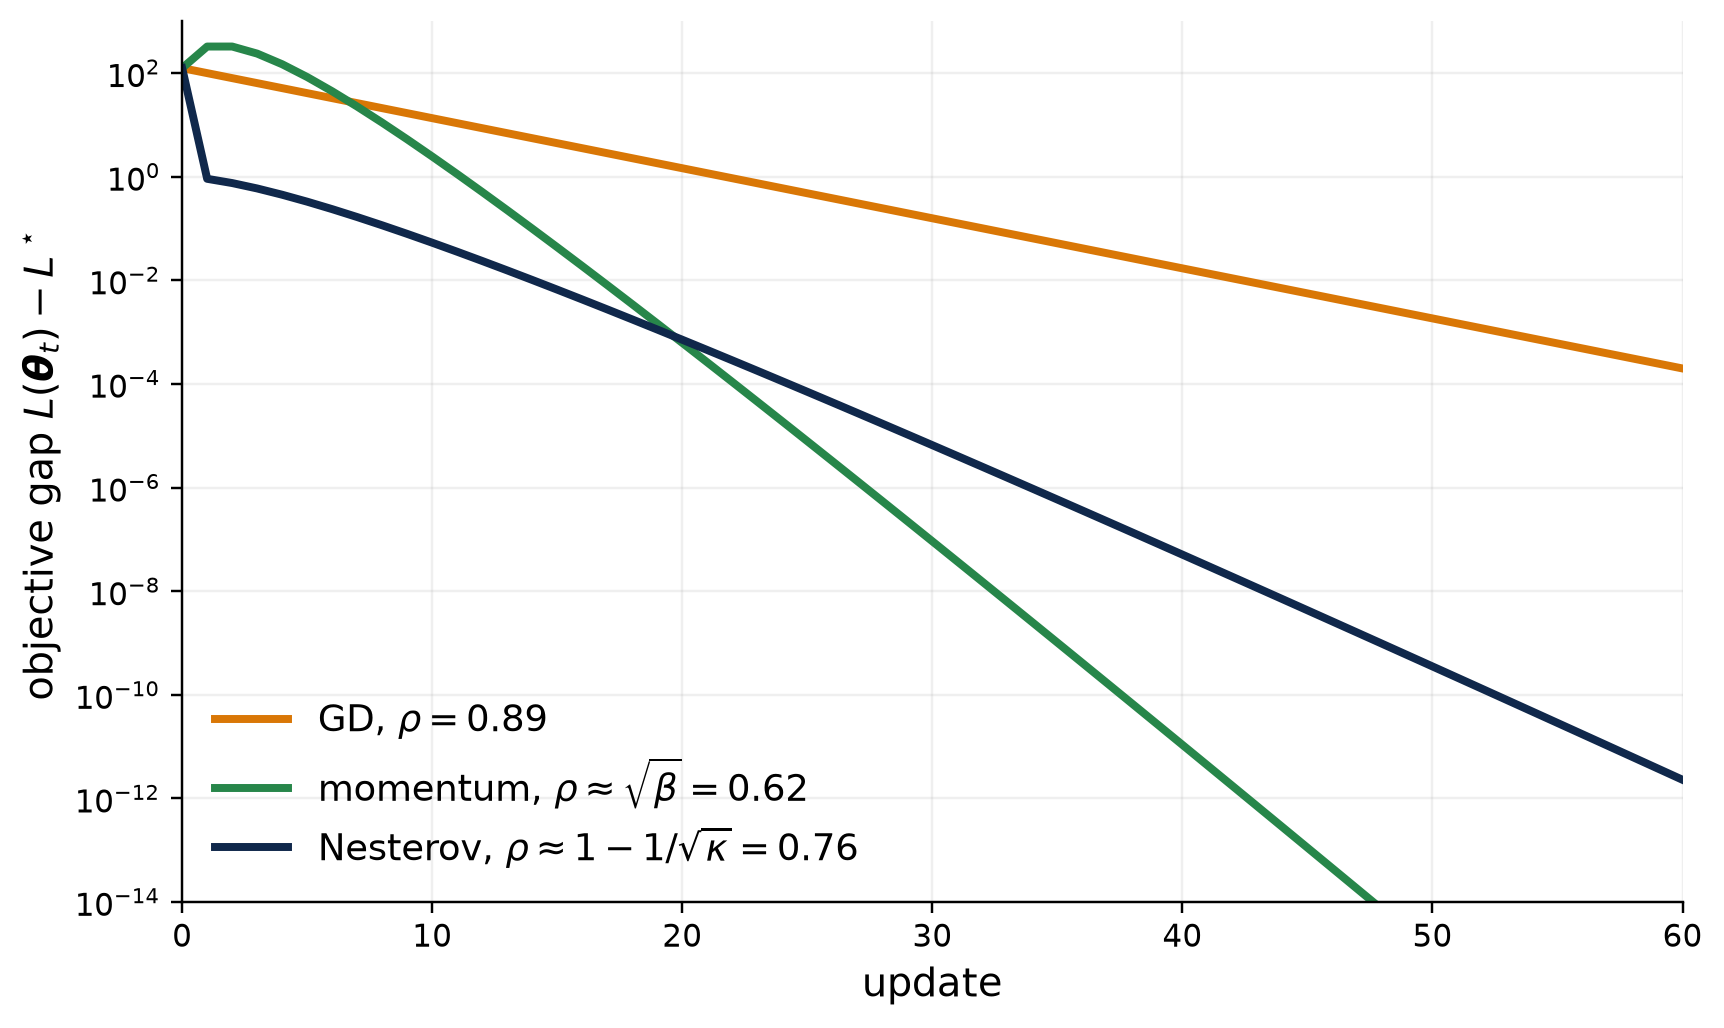
\includegraphics[width=0.66\linewidth,height=0.5\textheight,keepaspectratio]{momentum.png}

  \small
  Nesterov momentum takes the gradient where momentum alone would carry the iterate:
  $\mathbf g=\nabla L(\boldsymbol\theta-\eta\beta\mathbf v)$. On a quadratic with tuned parameters,
  momentum needs about $\sqrt\kappa$ updates where gradient descent needs about $\kappa$.
  The loss may rise at first: momentum does not decrease $L$ monotonically.
\end{frame}

\begin{frame}{Newton's Method and L-BFGS}
  \[
    \boldsymbol\theta^{(t+1)}=\boldsymbol\theta^{(t)}-\mathbf H^{-1}\nabla L(\boldsymbol\theta^{(t)})
  \]
  \begin{itemize}
    \item Newton's method divides the gradient by the curvature; on a quadratic it reaches the minimum in one update.
    \item It stores a $d\times d$ Hessian and solves a linear system, $O(d^3)$: impractical for millions of parameters.
    \item Where $\mathbf H$ has negative curvature (saddles) the step can point the wrong way.
    \item L-BFGS approximates it from the last few gradient differences; it suits smooth full-batch problems, not noisy mini-batches.
  \end{itemize}
\end{frame}

\begin{frame}{Gradient Clipping and Learning-Rate Search}
  \begin{itemize}
    \item \textbf{Clipping:} $\mathbf g\leftarrow\mathbf g\cdot\min(1,c/\|\mathbf g\|_2)$ keeps the direction and caps the step where the loss is very steep.
    \item \textbf{Learning-rate search:} try $\eta$ on a logarithmic grid for a short run; keep the largest value whose loss still decreases smoothly.
    \item A loss or gradient-norm spike calls for a smaller $\eta$ or a warm-up.
  \end{itemize}
\end{frame}

\begin{frame}{A Noiseless Quadratic Does Not Favor Adam}
  \centering
  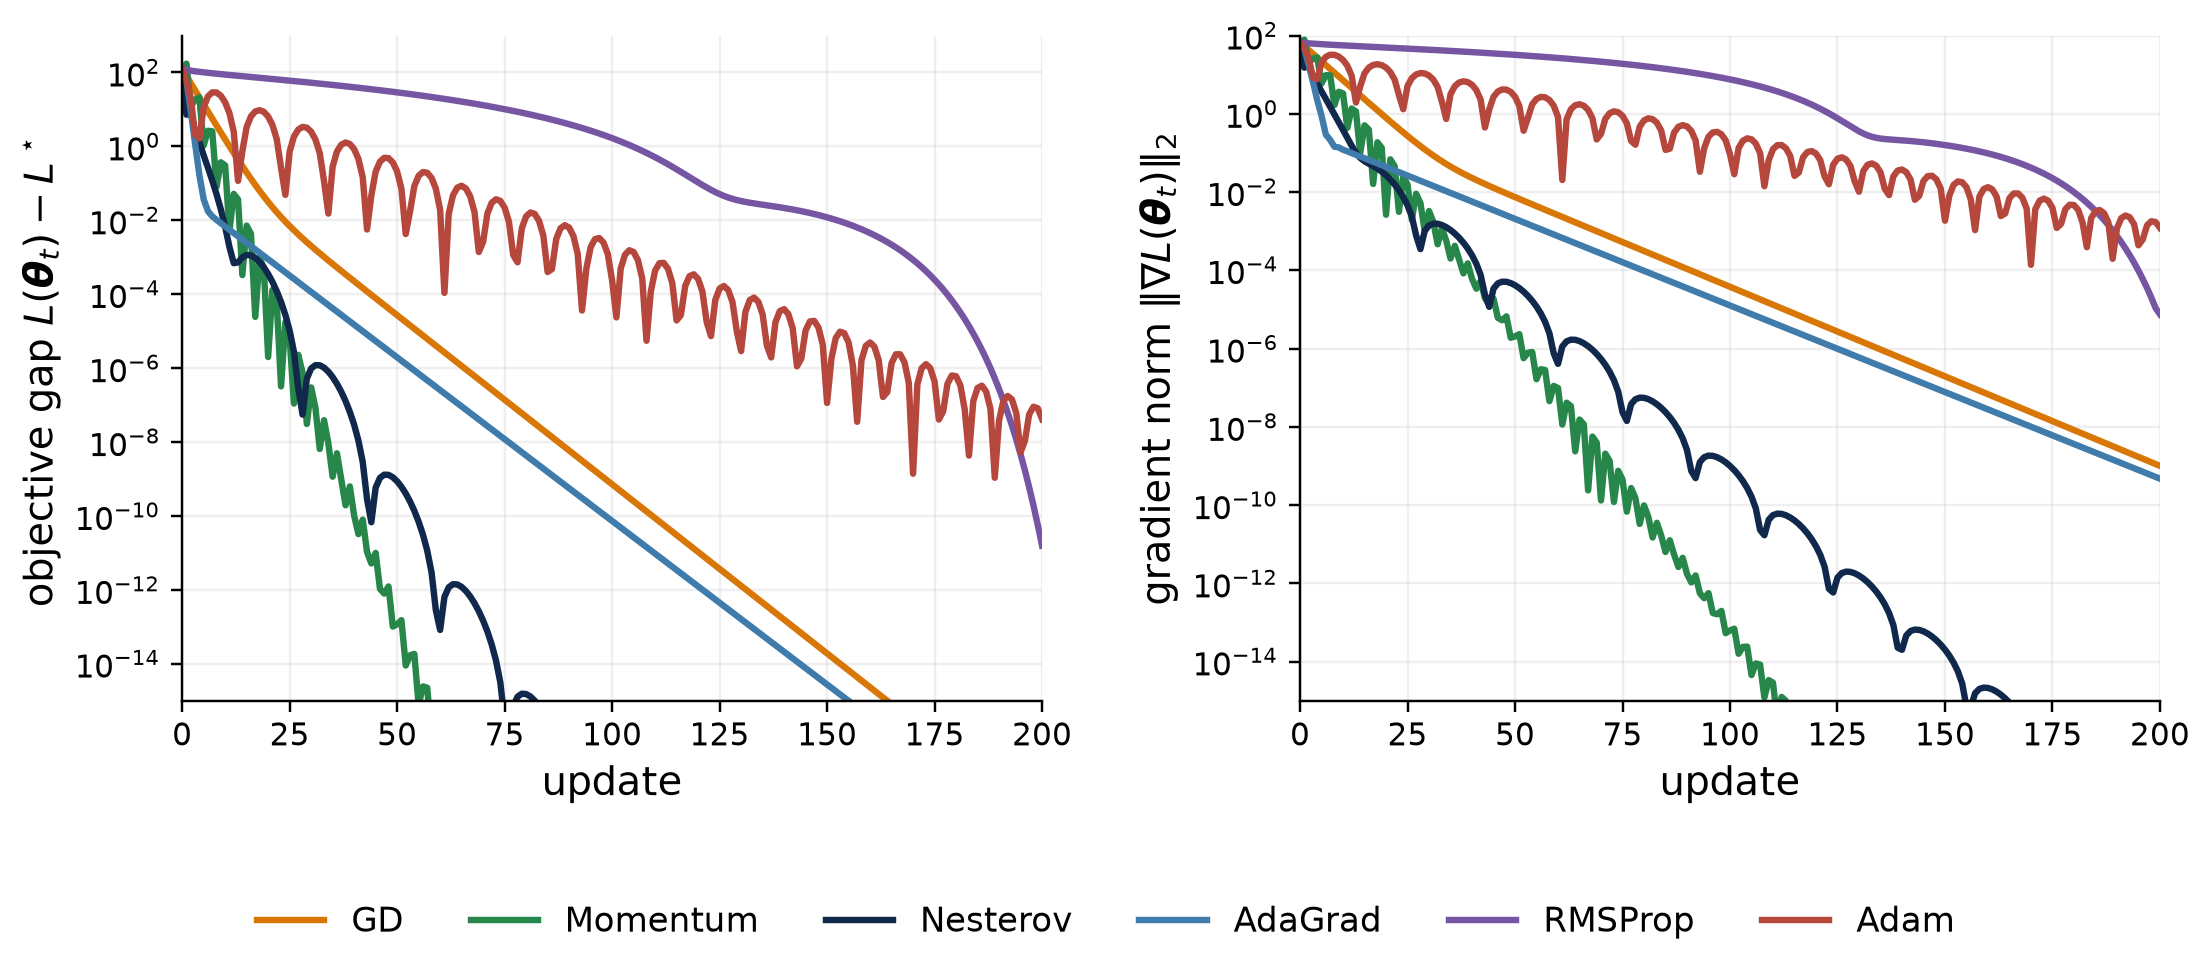
\includegraphics[width=0.96\linewidth,height=0.5\textheight,keepaspectratio]{optimizer-progress.png}

  \small
  Smooth quadratic, no noise, constant step tuned per method, 200 updates: GD, momentum and
  AdaGrad win; RMSProp and Adam hover near the minimum because their step stays about $\eta$
  in size. This is why Adam's advantages (noise, uneven scales, little tuning) must be shown on a
  problem that has them, as in the experiment above.
\end{frame}

\begin{frame}{Per-Parameter Scaling Does Not Fix Rotated Valleys}
  \centering
  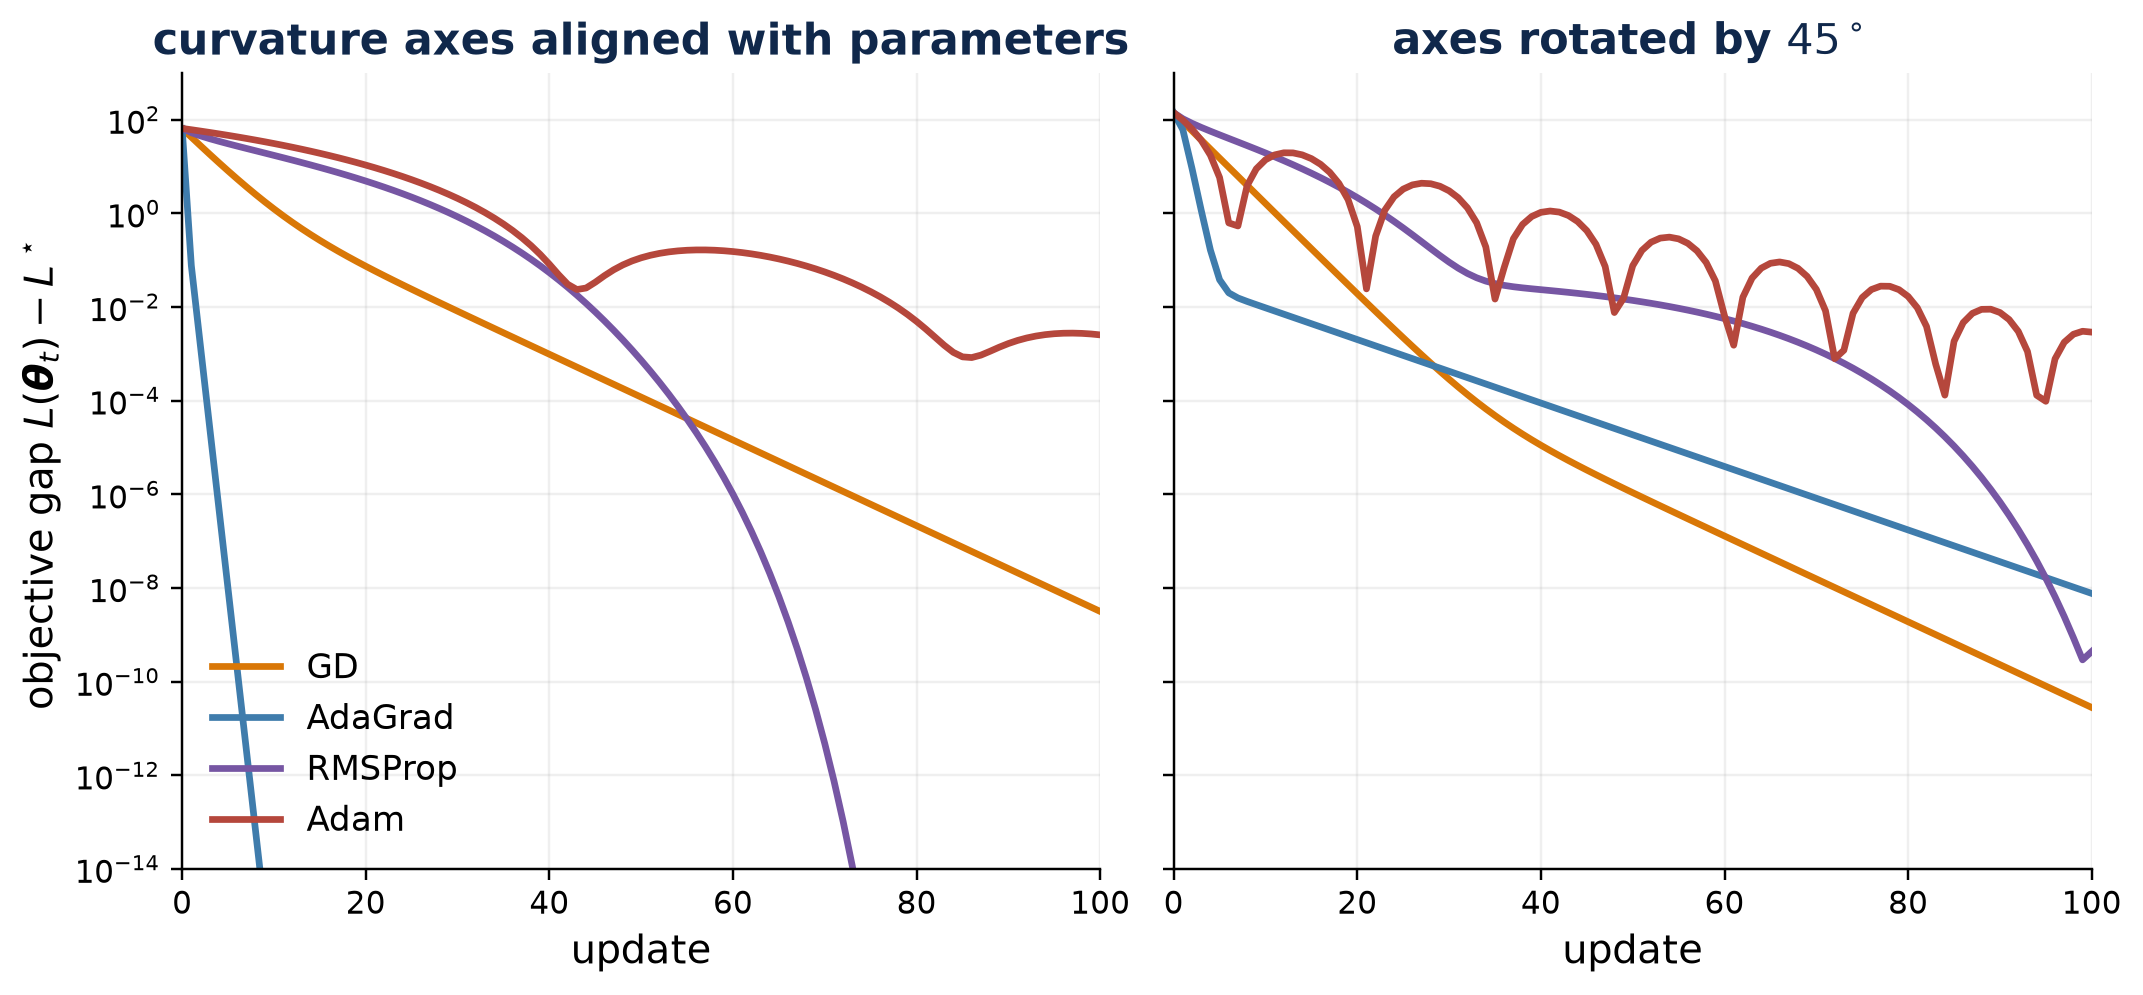
\includegraphics[width=0.98\linewidth,height=0.52\textheight,keepaspectratio]{diagonal-scaling.png}

  \small
  Dividing each coordinate separately only removes ill-conditioning that lies along the
  parameter axes (left). When the valley is rotated (right), it does not. Noiseless quadratic,
  each method tuned separately in each panel.
\end{frame}

\begin{frame}{A Curved Valley Rewards Momentum}
  \centering
  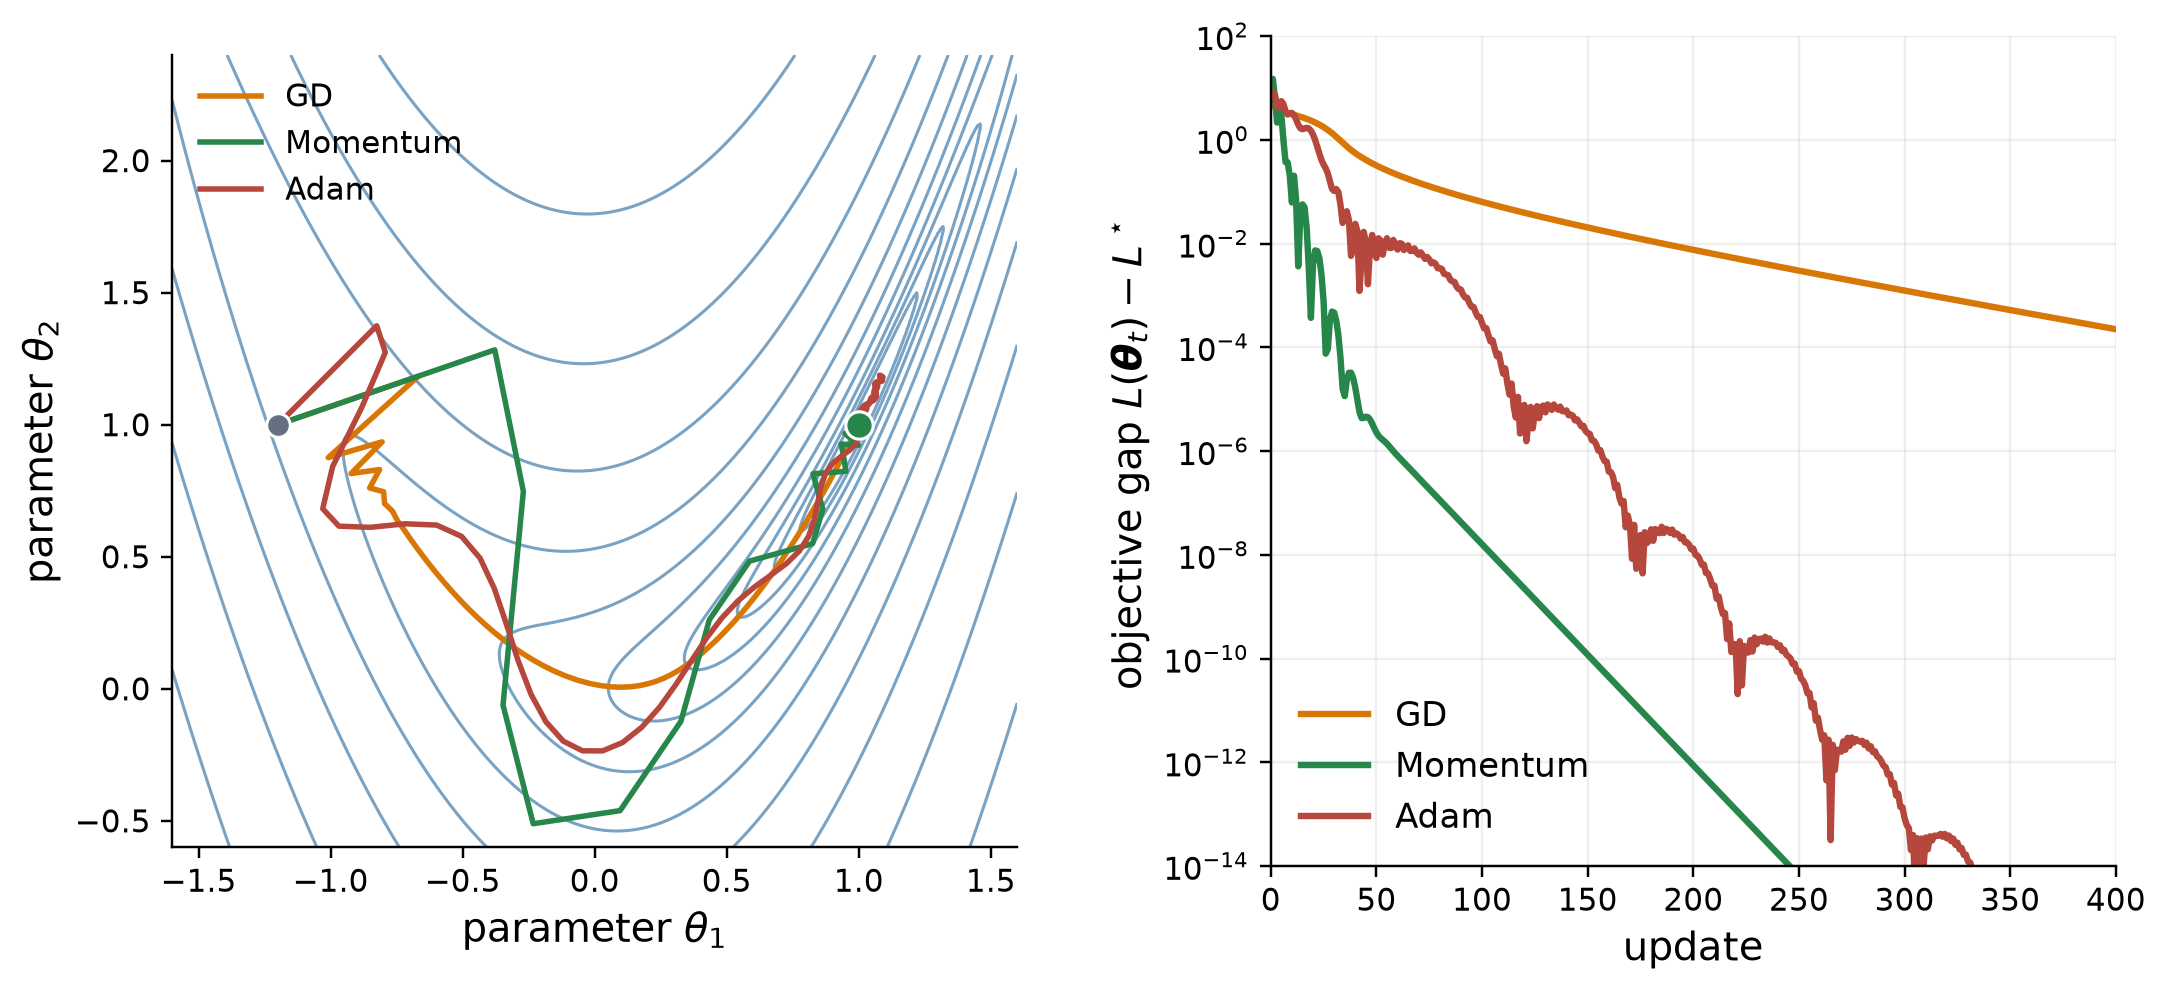
\includegraphics[width=0.96\linewidth,height=0.55\textheight,keepaspectratio]{rosenbrock.png}

  \small
  Rosenbrock's curved valley has a single minimum. Plain GD must keep $\eta$ small for the
  steep walls and crawls along the floor; momentum and Adam follow it faster.
\end{frame}

\begin{frame}{Leaving a Saddle}
  \centering
  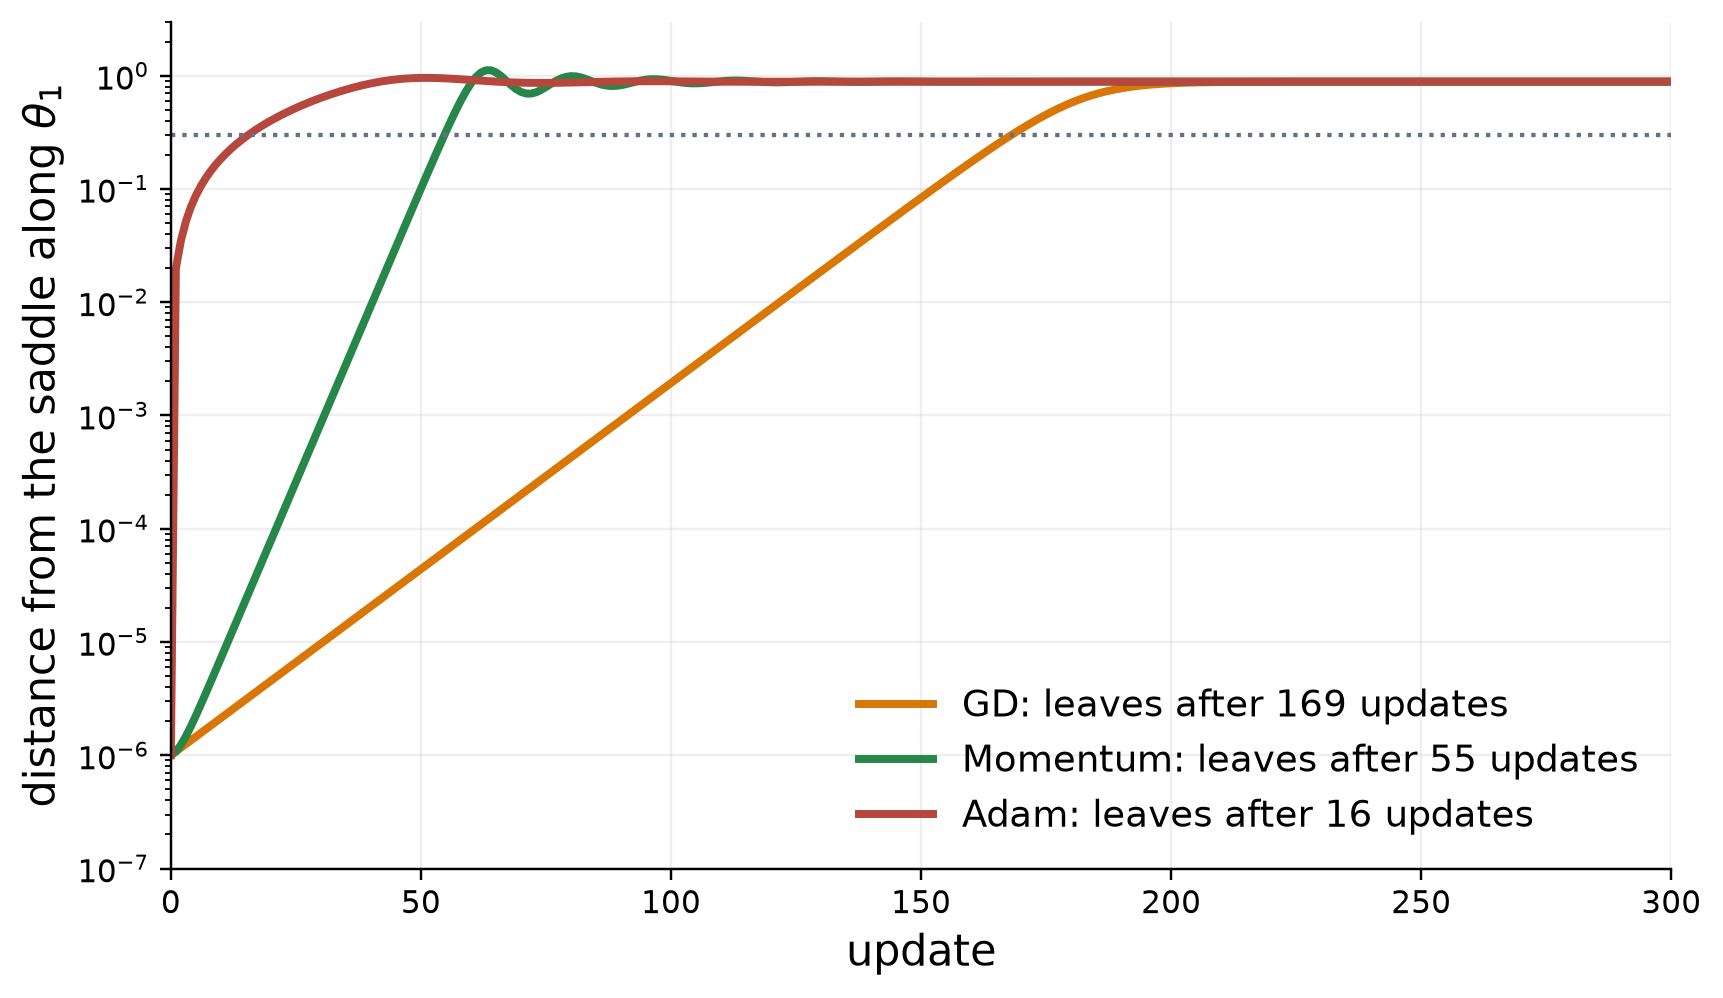
\includegraphics[width=0.8\linewidth,height=0.55\textheight,keepaspectratio]{saddle-escape.png}

  \small
  Near a saddle the gradient is tiny: GD's step shrinks with it, momentum accumulates it, and
  Adam divides by its own scale so its step stays near $\eta$ and it leaves soonest.
\end{frame}

\begin{frame}{The Start Decides Which Minimum Is Reached}
  \centering
  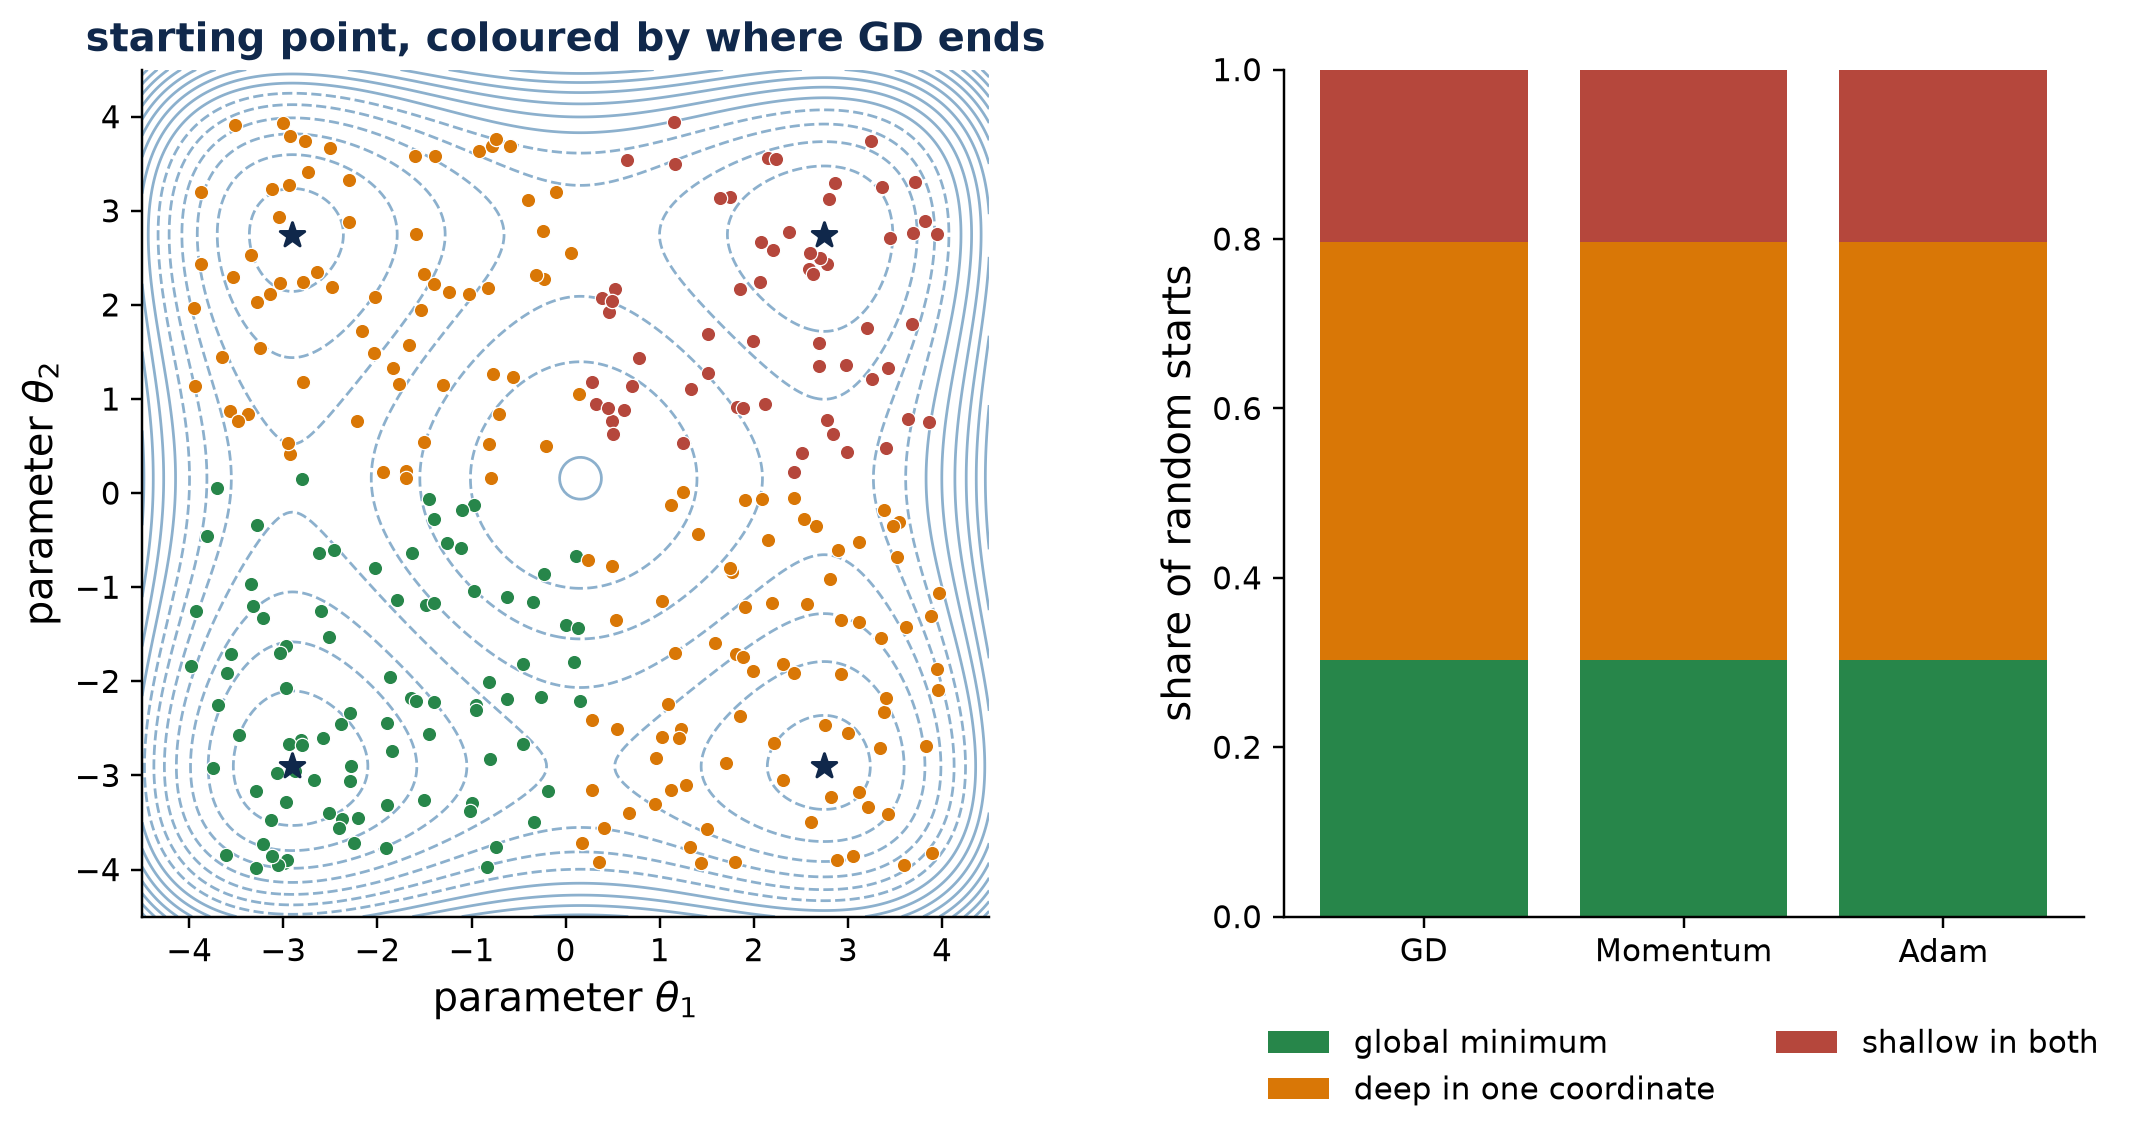
\includegraphics[width=0.9\linewidth,height=0.58\textheight,keepaspectratio]{multimodal.png}

  \small
  Four minima, one global. About $30\%$ of random starts reach the global one with every
  optimizer shown: none of these methods searches globally.
\end{frame}

\end{document}
